\chapter{Learning Stable Periodic Robot Motions from Demonstration}
\label{chp:osmp}

\begin{foreword}
    % So far, this thesis has focused mostly on the application of (learned) models within shape sensing and control. Yet, when working towards fully autonomous robots, one of the most challenging research topics is high-level decision making as the controllers that we have considered in this thesis all need either a setpoint or a trajectory to track. In Chapter~\ref{chp:braincontrol}, we introduced an approach to how users could directly control the robot with their thoughts by moving setpoints in space. However, while such low-level \gls{HRI} allows the human to control the robot's actions with vast detail, this requires the full attention of the user and is exhausting for the user, reducing some of the potential efficiency improvements that we envision robots to allow for. A promising alternative could be that the user communicates only high-level tasks to the robot, and the robot plans its motion by itself. Apart from \gls{RL} or optimization-based motion planning strategies such as \gls{MPC}, one of the most promising avenues here is \glsxtrfull{LFD}. Specifically, for 20 years, there has already been literature on learning motion policies with dynamical systems~\citep{ijspeert2013dynamical}, which the community refers to as \glsxtrfull{DMP}. In recent years, the advent of deep learning and normalizing flows~\citep{kobyzev2020normalizing} introduced the new concept of \glsxtrfull{SMP}, where a diffeomorphic mapping into latent space parametrized by a neural network is combined with a latent dynamical system~\citep{rana2020euclideanizing, perez2023stable, zhi2024teaching}. This allows the learning of more complex behaviors while preserving interpretability and stability guarantees. In this chapter, we extend the framework of \gls{SMP} to learning periodic motions while guaranteeing the orbital stability of the system.  We achieve this by combining a bijective encoder based on Euclideanizing flows with latent dynamics based on the supercritical Hopf bifurcation. This concept shares as similar spirit as in Chapter~\ref{chp:con}, although we now apply it to motion policies instead of learned dynamical models.
    % improved version by ChatGPT
    This thesis has so far concentrated primarily on the use of learned models in shape sensing and control. However, a critical challenge in achieving fully autonomous robots lies in high-level decision-making. The controllers discussed in this work require either a setpoint or a trajectory to follow. In Chapter~\ref{chp:braincontrol}, we explored a method enabling users to guide the soft robot directly through their thoughts by manipulating setpoints in space, which a compliant impedance controller subsequently tracks. While this low-level \gls{HRI} provides precise control over the robot’s actions, it demands the user’s full attention and can become exhausting, thereby limiting the efficiency gains we expect to gain by introducing intelligent, autonomous robots.
    %
    An alternative approach involves the user specifying only high-level tasks, allowing the robot to plan its motions independently. Among potential methods, including \gls{RL} and optimization-based strategies like \gls{MPC}, \gls{LFD} stands out as particularly promising as it allows the learning of complex motions from humans or even from other biological creatures. As a special case of \gls{LFD}, research on learning motion policies using dynamical systems has been well-established~\citep {ijspeert2013dynamical}. Being referred to as \glsxtrfull{DMP} or \glsxtrfull{SMP}, this strategy exhibits interpretability, compliant behavior, and convergence guarantees. Recently, advances in deep learning and normalizing flows~\citep{kobyzev2020normalizing} have given rise to frameworks that increase the expressiveness of the motion policy by leveraging diffeomorphic mappings into latent spaces, parametrized by neural networks, combined with latent dynamical systems~\citep{rana2020euclideanizing, perez2023stable, zhi2024teaching}. These methods enable the learning of more complex behaviors while maintaining interpretability, stability, and convergence guarantees.
    %
    In this chapter, we extend this approach to learn periodic motions with guaranteed orbital stability. This is achieved by integrating a bijective encoder based on Euclideanizing flows with latent dynamics modeled as supercritical Hopf bifurcations. The approach aligns in terms of vision with the work in Chapter~\ref{chp:con}, but here, it is applied to motion policy rather than dynamical model learning.
\end{foreword}

\pagebreak

\begin{abstract}
    % As we strive for humans and robots to collaborate closely or to have robots assist us in tasks of daily living, we need to make sure that the robots exhibit compliant, natural, and predictable behavior. 
    % Motion primitives represent velocity (or acceleration) fields that allow us to encode motions without any explicit time dependence and exhibit natural and compliant behaviors even under significant perturbations.
    % In recent years, there has been a strong push to leverage linear latent dynamics with a learned bijective encoder for learning stable, point-to-point motion primitives from demonstrations. However, existing approaches are not able to encode periodic motions.
    % In this work, we present how supercritical Hopf bifurcations in latent space allow for learning periodic motions from demonstration with stability guarantees. We introduce additional techniques such as phase synchronization, latent velocity shaping, and encoder conditioning that allow us to tackle complex, periodic robotic tasks such as turtle swimming or surface cleaning.
    % This will allow collaborative robots to perform periodic motions in an accurate, compliant, stable, and natural fashion and, with that, bring us one step closer to safe and intuitive human-robot collaboration.
    As we aim to foster closer collaboration between humans and robots—or to have robots assist us in everyday tasks—it is essential that these machines exhibit behavior that is robust, compliant, and natural. 
    Learning from demonstrations has proven to be a powerful approach for acquiring complex motion behaviors in a sample-efficient manner compared to methods like reinforcement learning.
    However, many current techniques—such as state-of-the-art diffusion policies—still require a large number of demonstrations to cover most state-action pairs, as these models lack inherent convergence guarantees.
    In contrast, dynamic motion primitives, which parameterize motion policies using dynamical systems, provide such convergence guarantees—often referred to as stable motion primitives—while maintaining natural and compliant behavior even under significant disturbances.
    Recent efforts have focused on leveraging linear latent dynamics paired with a learned, bijective encoder to derive stable, point-to-point motion primitives from demonstrations. However, these methods have fallen short when it comes to encoding periodic motions. In this work, we demonstrate that employing supercritical Hopf bifurcations in latent space can effectively learn periodic motions from demonstrations while ensuring stability. We further introduce techniques such as phase synchronization, online shaping of the convergence behavior, and encoder conditioning, which empower us to address complex periodic robotic tasks like turtle swimming and surface cleaning. These advancements pave the way for collaborative robots to perform periodic motions accurately, compliantly, stably, and naturally—bringing us one step closer to safe and intuitive human-robot interaction.
\end{abstract}

\blfootnote{This chapter is partly based on \faFileTextO ~\emph{\textbf{M. Stölzle}, T.K. Rusch*, Z.J. Patterson*, R. Pérez Dattari, F. Stella, J. Hughes, C. Della Santina, and D. Rus (2025). Learning Stable Periodic Robotic Motions from Demonstration. % In Science Robotics, 
\textbf{\emph{In Preparation}}}.
}

%% Start the actual chapter on a new page.
\newpage

\section{Introduction}

In recent years, \gls{IL}~\citep{schaal1999imitation, zare2024survey}, also often referred to as \gls{LFD} and, particularly, \gls{BC}, has gained significant momentum due to its sample and iteration efficiency in learning complex tasks, compared to alternatives such as \gls{RL}. The community has been focused on enhancing motion policies learned from demonstration to be more robust, high-performing, and generalizable by (i) integrating modern ML architectures like diffusion policies or flow matching to boost expressiveness and performance~\citep{chi2023diffusion, black2024pi0}, (ii) scaling up the number of demonstrations to improve robustness~\citep{o2024open, black2024pi0, gemini2025robotics}, (iii) training motion policies across multiple robot embodiments (e.g., various robotic manipulators) to enhance generalization~\citep{o2024open, black2024pi0}, and (iv) incorporating modern \glspl{VLM} whose embeddings serve as inputs to the motion policy, capturing both task and environmental state information~\citep{black2024pi0, kim2024openvla, gemini2025robotics}.

\glspl{DMP}~\citep{ijspeert2002learning, ijspeert2013dynamical, saveriano2023dynamic, hu2024fusion} parametrize a motion policy through dynamical systems that predict the desired velocity or acceleration based on the system’s current state. This approach offers several advantages: by grounding the formulation in dynamical systems, we can leverage established tools from nonlinear system theory~\citep{khalil2002nonlinear} to analyze behavior, and we can design these systems to ensure that the motion primitive exhibits stability and convergence guarantees—such as \gls{GAS}~\citep{ijspeert2013dynamical, rana2020euclideanizing, urain2020imitationflow, zhang2022learning, perez2023stable, perez2024puma} or \gls{OS}~\citep{ijspeert2002learning, khadivar2021learning, abu2024learning, zhi2024teaching}—which is not typically the case for standard ML-based motion policies like RNNs or Diffusion policies~\citep{chi2023diffusion, o2024open, black2024pi0, gemini2025robotics}.
These methods are sometimes referred to as \glspl{SMP}, and their robustness against perturbations, disturbances, and model mismatches arises because the motion policy continually steers the system back to the desired reference, even if it temporarily deviates from the demonstrated trajectory. Additionally, this characteristic leads to enhanced data efficiency, as it is not necessary to observe every possible state-action pair during training. Moreover, \glspl{DMP} have been shown to exhibit naturally compliant behavior~\citep{ijspeert2013dynamical, petrivc2018accelerated}, which reduces safety risks. While \glspl{DMP} can be conditioned on both time and system state, those not explicitly dependent on time are particularly interesting due to their natural and predictable response to perturbations~\citep{ijspeert2013dynamical}.

While there is a long history of research on \glspl{DMP}~\citep{ijspeert2002learning, ijspeert2013dynamical, saveriano2023dynamic, hu2024fusion}, their expressive power has traditionally been limited, preventing them from learning highly complex and intricate trajectories. Recently, however, an exciting research direction has emerged that combines diffeomorphisms into a latent space—learned using ML techniques—with relatively simple, analytically tractable (e.g., linear) latent space dynamics to enhance expressiveness while preserving stability and convergence guarantees~\citep{rana2020euclideanizing, urain2020imitationflow, zhang2022learning, perez2023stable}. Most of these works focus on point-to-point motions and aim to ensure \gls{GAS}~\citep{rana2020euclideanizing, zhang2022learning, perez2023stable, perez2024puma}. However, in our everyday lives, periodic or rhythmic motions (e.g., locomotion, cleaning movements) are ubiquitous. If we want robots to assist with daily tasks and exhibit robust athletic skills, we must develop techniques that encode such periodic motions into robot motion policies~\citep{ijspeert2002learning, ijspeert2013dynamical, khadivar2021learning, abu2024learning, zhi2024teaching}, ensuring orbital stability.

Recently, \citet{zhi2024teaching} took an important step by combining learned bijective encoders with a \emph{simple} latent space limit cycle to learn periodic trajectories from demonstrations while ensuring orbital stability for the motion policy within the proposed \gls{SPDT} approach. However, their method presents several limitations: (a) without a supervised imitation loss, it captures only the general direction of movement rather than the demonstrated velocities; (b) as shown in the paper, the approach only roughly approximates the demonstrated trajectory rather than replicating it accurately, likely due to the use of a Hausdorff distance~\citep{hausdorff1914grundzuge} loss; (c) the study focused on very simplified scenarios, with no verification on systems exceeding two Degrees of Freedom (DOFs); and (d) it does not offer solutions for many practical issues, such as synchronizing multiple systems—a common requirement in locomotion—or the ability to learn multiple distinct demonstrations within the same motion policy.

To address these shortcomings, we propose \glspl{OSMP}, which enable the learning of periodic motions from demonstrations while guaranteeing \gls{OS}. Similar to \citet{zhi2024teaching}, our approach combines a bijective encoder based on Euclideanizing flows~\citep{dinh2017density, rana2020euclideanizing} with a supercritical Hopf bifurcation~\citep{strogatz2018nonlinear} in latent space. This combination establishes an orbitally stable limit cycle while the neural network–based encoder provides the expressiveness required to learn complex, intricate motions.
First, to resolve issue (a), we incorporate an imitation loss that enables the model to learn the demonstrated velocities.
Second, unlike the method in~\citep{zhi2024teaching}, we introduce a limit cycle matching loss addressing limitation (b) that ensures the learned motion behavior closely mirrors the demonstration. 
In addressing (c), we validate our method in more complex scenarios—such as capturing both position and orientation evolution in systems with up to six DOFs. Finally, to counter (d), we propose strategies for (i) synchronizing multiple motion primitives while preserving their learned stable behavior and (ii) conditioning the encoder so that it can learn multiple demonstrations with diverse behaviors using the same neural network. The first strategy (i) allows us to synchronize the motion of two turtle robot limbs for effective swimming, while the second (ii) enables smooth interpolation between learned behaviors, such as seamlessly transitioning between forward and reverse swimming modes.

We conduct extensive verification of our proposed approach in both simulation and real-world scenarios. First, we benchmark our method both quantitatively and qualitatively against several baselines, including traditional machine learning techniques like \glspl{RNN} and \glspl{NODE}~\citep{zhi2024teaching}, as well as the diagrammatic teaching method by \citet{zhi2024teaching}. Second, we demonstrate experimentally that the orbital motion primitives enable accurate and stable trajectory tracking across a diverse range of robotic systems—including robotic manipulators (UR5), cobots (KUKA), soft robots (Helix Robot)~\citep{guan2023trimmed}, and hybrid underwater robots (crush turtle robot developed by the Distributed Robotics Lab at MIT). Third, we confirm that this motion learning approach effectively handles cleaning tasks demonstrated via kinesthetic teaching. Fourth, we show that parameterizing the learned motion policies with dynamical systems, without any explicit time dependence, yields more compliant and natural behavior compared to traditional error-based feedback controllers operating on time-parametrized trajectories. Fifth, we illustrate the synchronization of multiple \glspl{OSMP} to operate in phase. Finally, we demonstrate that encoder conditioning enables a single \gls{OSMP} to learn multiple distinct motion modes, allowing smooth interpolation between these modes at inference time.

\section{Methodology}

In this work, we introduce \glspl{OSMP}, which can be trained to capture complex periodic motions from demonstrations while ensuring convergence to a limit cycle that aligns with a predefined oracle. To accomplish this, we build on previous research~\citep{rana2020euclideanizing, zhi2024teaching} that combines learned bijective encoders with a prescribed motion behavior in latent space. These latent dynamics generate velocities or accelerations that are subsequently mapped back into the oracle space via a pullback operator~\citep{zhang2022learning}—in the case of a bijective encoder, this operator is the inverse of the encoder’s Jacobian. In this formulation, the motion in latent space exhibits key convergence properties, such as Global Asymptotic Stability (GAS)~\citep{rana2020euclideanizing, perez2023stable, sochopoulos2024learning} or Orbital Stability (OS)~\citep{zhi2024teaching}, while the learned encoder provides the necessary expressiveness to capture complex motions and transfers the convergence guarantees from latent to oracle space through the established diffeomorphism.

However, compared to existing work~\citep{zhi2024teaching}, we introduce several crucial modifications that enhance both the performance and practical utility of the proposed method: (1) we develop a limit cycle matching loss to reduce the discrepancy between the learned limit cycle and the periodic oracle; (2) we design strategies to modulate the learned velocity field online without the need for retraining—for instance, to adjust the convergence behavior; (3) we establish a procedure to synchronize the phase of multiple \glspl{OSMP}; and (4) we condition the encoder on a task, enabling a single \gls{OSMP} to exhibit multiple distinct motion behaviors. Moreover, we introduce loss terms that allow the trained \gls{OSMP} to smoothly interpolate between the learned motion behaviors—something that has not been possible before.

\subsection{Orbitally Stable Motion Primitives}
The dynamical motion policy $\dot{x}=f(x; z)$ is typically defined in task space but can also be defined in other Cartesian or generalized coordinates (e.g., joint space). Therefore, we will in the following refer to these coordinates as \emph{Oracle space}.
In this work, we are specifically interested in cases where we train $f(x)$ to learn periodic motions.
Then, the smooth diffeomorphism between the oracle and latent space is made via a bijective encoder $\Psi: \mathbb{R}^n \to \mathbb{R}^n$, which maps positional states $x \in \mathbb{R}^n$ into the latent states $y \in \mathbb{R}^n$.
Optionally, this encoding is conditioned on a continuous variable $z \in \mathbb{R}$ as a homotopy such that $y = \Psi(x;z)$.
Furthermore, we construct $\Psi$ such that it is invertible and a closed-form inverse function $\Psi^{-1}: y \mapsto x$ allows us to map from latent space back into oracle space.
In latent space, we apply dynamics $\dot{y} = f_\mathrm{y}(y)$ that exhibit a stable limit cycle behavior. In summary, the orbitally stable motion primitive is given as
\begin{equation}\label{eq:dynamics}
    \dot{x} = f(x;z) = f_\mathrm{s}(x) \, J_\Psi^{-1}(x;z) \, f_\mathrm{y} \left (\Psi(x;z) \right ),
\end{equation}\
where $J_\Psi = \frac{\partial \Psi(x;z)}{\partial x}$ defines the Jacobian of the encoder. 
The function $f_\mathrm{s}(x): \mathbb{R}^n \to \mathbb{R}_{>0}$ scales the velocity magnitude and is implemented as $f_\mathrm{s}(x) = e^{\mathrm{MLP}(x)} + \varepsilon$, where $\varepsilon \in \mathbb{R}_{>0}$ is a small value~\citep{rana2020euclideanizing}.
As $\Psi$ is a diffeomorphism (w.r.t. $x$ and $y$), the motion policy is orbitally stable by construction~\citep{rana2020euclideanizing, zhi2024teaching}.

\subsubsection{Diffeomorphic Encoder}
We consider a bijective encoder $\Psi_\theta : \mathbb{R}^n \times \mathbb{R} \to \mathbb{R}^n$, which maps positional states $x \in \mathbb{R}^n$ into the latent states $y \in \mathbb{R}^n$ conditioned on $z \in \mathbb{R}$, where we assume that $n \in \mathbb{N} \geq 2$.
The encoder $y = \Psi_\theta(x;z)$ adopting the Euclideanizing flows~\citep{dinh2017density, rana2020euclideanizing} architecture is parametrized by the learnable weights $\theta \in \mathbb{R}^{n_\theta}$ and consists of $n_\mathrm{b}$ blocks, where each block is analytically invertible.
If a conditioning is used, $z$ is first lifted into an embedding $\Bar{z}$, which is subsequently used to condition each block.
More details on the encoder architecture can be found in the pioneering work~\citep{dinh2017density, rana2020euclideanizing} and Section~\ref{sub:osmp:methodology:training}.

\subsubsection{Latent Dynamics}
In latent space, we consider the 1st-order dynamics of a supercritical Hopf bifurcation~\citep{strogatz2018nonlinear, khadivar2021learning, zhi2024teaching, nah2025combining}
\begin{equation}\label{eq:osmp:latent_dynamics}
    \dot{y} = \begin{bmatrix}
        \dot{y}_1\\
        \dot{y}_2\\
        \dot{y}_{3:n}\\
    \end{bmatrix} = f_\mathrm{y}(y) = \begin{bmatrix}
        -\omega(y) \, y_2 + \alpha \, \left ( 1 - \frac{y_1^2 + y_2^2}{R^2} \right ) \, y_1\\
        + \omega(y) \, y_1 + \alpha \, \left ( 1 - \frac{y_1^2 + y_2^2}{R^2} \right ) \, y_2\\
        -\beta \, y_{3:n}\\
    \end{bmatrix},
    % \quad
    % \forall i \: \in 3, \dots, N.
\end{equation}
where $\omega(y) = f_\omega(\operatorname{atan2}(y_2, y_1)) > 0$ determines the angular velocity.
Here, the dynamics of $y_1$ and $y_2$ describe the Cartesian-space behavior of a simple limit cycle whose behavior in polar coordinates $y_\mathrm{pol} = \begin{bmatrix}
    r & \varphi & y_{3:n}^\top
\end{bmatrix}^\top$ is expressed as
\begin{equation}\label{eq:osmp:latent_dynamics_polar_coordinates}
    \dot{y}_\mathrm{pol} = \begin{bmatrix}
        \dot{r}\\ \dot{\varphi}\\ \dot{y}_{3:n}
    \end{bmatrix} = f_\mathrm{pol}(y_\mathrm{pol}) = \begin{bmatrix}
        \alpha \left ( 1 - \frac{r^2}{R^2} \right ) \, r\\ f_\omega(\varphi)\\ -\beta \, y_{3:n}\\
    \end{bmatrix},
    % \quad
    % \forall i \: \in 3, \dots, N,
\end{equation}
where $f_\omega(\varphi): [-\pi, \pi) \to \mathbb{R}_{>0}$ computes the positive angular velocity as a function of the polar angle. Often, in particular, when employing $f_\mathrm{s}(x) \neq 1$, it can also be set to a constant: $\omega = 1$. 
If not, we define in practice $\omega(y) = f_\omega(\Bar{y}_{1:2}) = e^{\mathrm{MLP}(\Bar{y}_{1:2})} + \epsilon_\omega$, where $\Bar{y}_{1:2} = \begin{bmatrix}
    \frac{y_1}{\sqrt{y_1^2+y_2^2}} &  \frac{y_2}{\sqrt{y_1^2+y_2^2}}
\end{bmatrix}^\top \in \mathbb{R}^2$ with $\epsilon_\omega > 0$.

$\alpha > 0$ and $\beta > 0$ are positive gains that determine how fast the system converges onto the limit cycle.  When learning the dynamics, we choose $\alpha = \beta = 1$. $R \in \mathbb{R}_{>0}$ expresses the radius of the limit cycle in latent space. Again, it is sufficient to choose $R =1$ or $R=0.5$.
% Finally, latent space velocity is mapped back into the original space using the inverse Jacobian of the encoder $\dot{x} = J_\Psi^{-1} \, \dot{y}$.

\paragraph{Map from Polar to Cartesian Coordinates}
The map $h_{\mathrm{p2y}}(y_\mathrm{pol}): \mathbb{R}^n \to \mathbb{R}^n$ from latent polar coordinates to latent Cartesian coordinates and its inverse $h_{\mathrm{y2p}}(y) = h_{\mathrm{p2y}}^{-1}(y)$ is given by
\begin{equation}
    y = h_{\mathrm{p2c}}(y_\mathrm{pol}) = \begin{bmatrix}
        r \, \cos(\varphi)\\
        r \, \sin(\varphi)\\
        y_{3:n}
    \end{bmatrix},
    \qquad
    y_\mathrm{pol} = h_{\mathrm{c2p}}(y) = \begin{bmatrix}
        \sqrt{y_1^2+y_2^2}\\
        \operatorname{atan2}(y_2, y_1)\\
        y_{3:n}
    \end{bmatrix}.
\end{equation}
Then, the Jacobian of the Polar-to-Cartesian map $\frac{\partial h_{\mathrm{p2c}}}{\partial y_\mathrm{pol}} \in \mathbb{R}^{n \times n}$ is given by
\begin{equation}
    \frac{\partial h_{\mathrm{p2c}}}{\partial y_\mathrm{pol}} = \begin{bmatrix}
        \cos(\varphi) & -r \, \sin(\varphi) & 0_{1 \times (n-2)}\\
        \sin(\varphi) & r \, \cos(\varphi) & 0_{1 \times (n-2)}\\
        0_{(n-2) \times 1} & 0_{(n-2) \times 1} & \mathbb{I}_{n-2}
    \end{bmatrix}
\end{equation}
We can also substitute $y_\mathrm{pol} = y$ into the Jacobian and determine its inverse
\begin{equation}
    \frac{\partial h_{\mathrm{p2c}}}{\partial y_\mathrm{pol}} = \begin{bmatrix}
        \frac{y_1}{\sqrt{y_1^2 + y_2^2}} & -y_2 & 0_{1 \times (n-2)}\\
        \frac{y_2}{\sqrt{y_1^2 + y_2^2}} & y_1 & 0_{1 \times (n-2)}\\
        0_{(n-2) \times 1} & 0_{(n-2) \times 1} & \mathbb{I}_{n-2}
    \end{bmatrix},
    \qquad
    \frac{\partial h_{\mathrm{p2c}}}{\partial y_\mathrm{pol}}^{-1} = \begin{bmatrix}
        \frac{y_1}{\sqrt{y_1^2 + y_2^2}} & \frac{y_2}{\sqrt{y_1^2 + y_2^2}} & 0_{1 \times (n-2)}\\
        -\frac{y_2}{y_1^2 + y_2^2} & \frac{y_1}{y_1^2 + y_2^2} & 0_{1 \times (n-2)}\\
        0_{(n-2) \times 1} & 0_{(n-2) \times 1} & \mathbb{I}_{n-2}
    \end{bmatrix},
\end{equation}
which are both full-rank for $r = \sqrt{y_1^2 + y_2^2} > 0$.

\subsection{Training}\label{sub:osmp:methodology:training}
We consider a dataset $\langle T, X^\mathrm{d}, \dot{X}^\mathrm{d}, Z \rangle$ as a tuple between timestamps $T = \langle t(1), \dots, t(k), \dots, t(N) \rangle$ positions $X^\mathrm{d} = \langle x^\mathrm{d}(1), \dots, x^\mathrm{d}(k), \dots, x^\mathrm{d}(\mathrm{N}) \rangle$, the corresponding, demonstrated velocities $\dot{X}^\mathrm{d} = \langle \dot{x}^\mathrm{d}(1), \dots, \dot{x}^\mathrm{d}(k), \dots, \dot{x}^\mathrm{d}(\mathrm{N}) \rangle$ and an optional conditioning $Z = \langle z(1), \dots, z(k), \dots, z(\mathrm{N}) \rangle$, where $k \in \mathbb{N}_\mathrm{N} = \{1, 2, \dots, N \}$.
%

\subsubsection{Bijective Encoder}
The bijective encoder based on Euclideanizing flow~\citep{rana2020euclideanizing} / Real NVP~\citep{dinh2017density} uses coupling layers with the scaling and translation functions parametrized by \glspl{RFFN} that integrate ELU activation functions and a hidden dimension of $100$.
The number of encoder layers/blocks varies by the complexity of the task and ranges from $10$ for simple tasks to $25$ for very complex tasks.
At the start of the training, the encoder is initialized as an identity mapping.

\subsubsection{(Angular) Velocity Scaling Network}
The optional velocity scaling network $e^{\mathrm{MLP}(x)}$ is parametrized by a three-to-five-layer MLP (depending on the nonlinearities and discontinuities that the demonstration velocity profile exhibits) with a hidden dimension of $128$ and LeakyReLU activation functions.

Similarly, the angular velocity network $\omega(y) = f_\omega(\Bar{y}_{1:2}) = e^{\mathrm{MLP}(\Bar{y}_{1:2})} + \epsilon_\omega$, where $\Bar{y}_{1:2} = \begin{bmatrix}
    \frac{y_1}{\sqrt{y_1^2+y_2^2}} &  \frac{y_2}{\sqrt{y_1^2+y_2^2}}
\end{bmatrix}^\top \in \mathbb{R}^2$ with $\epsilon_\omega = 10^{-6}$, is parametrized by a five-layer MLP with a hidden dimension of $128$ and LeakyReLU activation functions.

\subsubsection{Loss Functions}
The total training loss function is then given by
\begin{equation}
    \mathcal{L} = \underbrace{\zeta_\mathrm{vi} \, \mathcal{L}_\mathrm{vi}}_\text{Vel. Imitation} + \underbrace{\zeta_\mathrm{lcm} \, \mathcal{L}_\mathrm{lcm}}_\text{Limit Cycle Matching} + \underbrace{\zeta_\mathrm{tgd} \, \mathcal{L}_\mathrm{tgd}}_\text{Time Guidance} 
    + \underbrace{\zeta_\mathrm{er} \, \mathcal{L}_{\mathrm{er}}}_\text{Encoder Reg.}
    + \underbrace{\zeta_\mathrm{vr} \, \mathcal{L}_{\mathrm{vr}}}_\text{Vel. Reg.}  + \underbrace{\zeta_\mathrm{sci} \, \mathcal{L}_{\mathrm{sci}}}_\text{Cond. Interpolation} 
    % + \underbrace{\zeta_\mathrm{wr} \, \mathcal{L}_\mathrm{wr}}_\text{NN Weight Reg.},
\end{equation}
where $\zeta_\mathrm{vi}, \zeta_\mathrm{lcm}, \zeta_\mathrm{tgd}, \zeta_\mathrm{er}, \zeta_\mathrm{vr}, \zeta_\mathrm{sci} \in \mathbb{R}$ are scalar loss weights.
$\mathcal{L}_\mathrm{vi}$ is a loss term that enforces that the velocity of the motion primitive matches the one demanded by the demonstration at all samples in the demonstration dataset, $\mathcal{L}_\mathrm{lcm}$ ensures that the encoded demonstration positions lie on the latent limit cycle. The time-guidance loss $\mathcal{L}_\mathrm{tgd}$ can support the limit cycle matching loss for highly curved demonstrations. 
The term $\mathcal{L}_\mathrm{er}$ regularizes the encoder by penalizing deviations from the identity encoder.
The optional $\mathcal{L}_{\mathrm{sci}}$ gives rise to smooth interpolation between different encoder conditioning.
% , and $\mathcal{L}_\mathrm{wr}$ regularizes the encoder network weights.
The discretionary velocity regularization loss $\zeta_\mathrm{vr}$ increases the numerical stability by penalizing very high velocities. In the following, we define each loss term formally.

\paragraph{Velocity Imitation Loss}
Analog to the literature on stable point-to-point motion primitives~\citep{rana2020euclideanizing}, the predicted oracle space velocity is supervised by a smooth $\ell_1$ loss~\citep{girshick2015fast}, which computes a squared term if the absolute error falls below $\beta_{\ell_1}$ and the $\ell_1$ term otherwise, and can be formally defined as
\begin{equation}
    % \mathcal{L}_\mathrm{vi} = \sum_{k = 1}^{N} \frac{\lVert \dot{x}^\mathrm{d}(k) - f(x^\mathrm{d}(k);z(k)) \rVert_2^2}{N}.
    \mathcal{L}_\mathrm{vi} = \frac{1}{N} \, \sum_{k = 1}^{N} \begin{cases}
		\frac{\left ( f(x^\mathrm{d}(k);z(k)) - \dot{x}^\mathrm{d}(k) \right )^2}{2 \, \ell_1}, & \text{if} \: \left \lVert f(x^\mathrm{d}(k);z(k)) - \dot{x}^\mathrm{d}(k) \right \rVert_1 < \beta_{\ell_1} \\
        \left \lVert f(x^\mathrm{d}(k);z(k)) - \dot{x}^\mathrm{d}(k) \right \rVert_1 - \frac{\beta_{\ell_1}}{2} , & \text{otherwise}
    \end{cases},
\end{equation}
where we choose $\beta_{\ell_1} = 1$.

\paragraph{Limit Cycle Matching Loss}
Next, we consider a subset of the demonstrations $\mathcal{P} \subset \mathbb{N}_\mathrm{N}$ that exhibit a periodic motion. To guarantee the OS of the learned system, we need to make sure that the learned limit cycle matches the periodic demonstration.
For this purpose, we design a \emph{limit cycle matching} loss $\mathcal{L}_\mathrm{lcm}$ in latent space
% \begin{equation}
% \begin{split}
%     y_\mathrm{p}(k) =& \: \begin{bmatrix}
%         \sqrt{y_1^2(k) + y_2^2(k)} & y_3 & \dots & y_n
%     \end{bmatrix}^\mathrm{T}, \\
%     y_\mathrm{p}^\mathrm{d}(k) =& \: \begin{bmatrix}
%         R & 0 & \dots & 0
%     \end{bmatrix}^\mathrm{T}, \\
%     \mathcal{L}_\mathrm{lcm} =& \: \sum_{k \in \mathcal{P}} \frac{\big \lVert y_\mathrm{p}^\mathrm{d}(k) - y_\mathrm{p}(k) \big \rVert_2^2}{|\mathcal{P}|},
% \end{split}
% \end{equation}
\begin{equation}\small
    y_\mathrm{p}(k) = \begin{bmatrix}
        \sqrt{y_1^2(k) + y_2^2(k)}\\ y_{3:n}
    \end{bmatrix} \in \mathbb{R}^{n-1},
    \quad
    y_\mathrm{p}^\mathrm{d}(k) = \begin{bmatrix}
        R\\ 0_{n-2}
    \end{bmatrix},
    \quad
    \mathcal{L}_\mathrm{lcm} = \sum_{k \in \mathcal{P}} \frac{\big \lVert y_\mathrm{p}^\mathrm{d}(k) - y_\mathrm{p}(k) \big \rVert_2^2}{|\mathcal{P}|},
\end{equation}
where $|\mathcal{P}|$ is the cardinality of $\mathcal{P}$, and $y=\Psi(x^\mathrm{d}; z) \in \mathbb{R}^n$ is the latent encoding. % , and $y_\mathrm{p}^\mathrm{d}$ and $y_\mathrm{p}$ are the desired and actual latent positions in polar coordinates, respectively.

\paragraph{Time Reference Guidance Loss}
% For highly curved oracles, we found it to be helpful to guide the mapping of the oracle positions onto latent polar angle by leveraging the time parametrization of the oracle. The idea is to evenly distribute the oracle positions onto the latent-space limit cycle and preventing the encoders to be clustered in one region of the latent limit cycle while other polar angular regions do not have a correspondence on the oracle.
For strongly curved oracles, we have found it advantageous to use the oracle’s time parameterization to steer how its positions map onto the latent polar angle. Doing so spreads the oracle samples uniformly around the latent-space limit cycle, preventing the encoders from bunching up in one angular sector while leaving other portions of the cycle without corresponding oracle points.

First, we compute for each position contained in the rhythmic demonstration a desired latent polar angle based on the normalized time reference. Simultaneously, we evaluate the actual encoded polar angle of $x^\mathrm{d}(k)$ as
\begin{equation}
     \varphi^\mathrm{d}(k) = \varphi_0 + 2 \, \pi \, \frac{t(k)}{P},
     \qquad
     \varphi(k) = \operatorname{atan2}\left ( \Psi(x(k);z(k))_2, \{ \Psi(x(k);z(k)) \}_1 \right),
\end{equation}
where $\varphi_0$ is the polar angle anchor and $P$ is the period of the rhythmic demonstration.
Subsequently, we define a positive alignment loss between the 
\begin{equation}
    \mathcal{L}_\mathrm{tgd} = \sum_{k \in \mathcal{P}} \frac{\max \left ( \left | \operatorname{mod} \bigl( \varphi^\mathrm{d}(k) - \varphi(k) + \pi,\; 2\pi\bigr) - \pi \right | - m_\mathrm{tgd}, 0 \right )^2}{|\mathcal{P}|},
\end{equation}
$m_\mathrm{tgd} \in \mathbb{R}_{>0}$ is the allowed margin between the time reference and the actual polar phase and the function $n_{e_\varphi}(e_\varphi) = \operatorname{mod} \bigl( e_\varphi(k) + \pi,\; 2\pi\bigr) - \pi$ normalizes the polar angle error $e_\varphi(k) = \varphi^\mathrm{d}(k) - \varphi(k) $ into the interval $[-\pi, \pi)$.

\paragraph{Encoder Regularization}
Similar to Zhi \textit{et al.}~\citep{zhi2024teaching}, we employ an encoder regularization loss $\mathcal{L}_{\Psi, \mathrm{reg}}$ that penalizes deviations from an identity encoder $y = \Psi(x) = x$.
We draw in each epoch $N$ random positions samples $x(k) ~\sim \mathcal{U}(x_\mathrm{min}, x_\mathrm{max}) \: \forall \, k \in \mathbb{N}_N$ from a uniform distribution within the workspace $[x_\mathrm{min}, x_\mathrm{max}]$ of the system. Then, the loss is computed as
\begin{equation}
    \mathcal{L}_{\mathrm{er}} = \sum_{k=1}^{N} \frac{\lVert x - \Psi(x;z) \rVert}{N}.
\end{equation}


\paragraph{Velocity Regularization}
% The velocity imitation loss $\mathcal{L}_\mathrm{vi}$ only supervises the velocity on the demonstration. However, in particular in cases with very few demonstrations that are close to each other, the velocity magnitude remains unsupervised in many parts of the system workspace, even though orbital stability and transverse contraction always remains ensured. However, in practice, large predicted velocities frequently lead to numerical instability. Therefore, it can be helpful to regularize the predicted velocities.
The velocity-imitation loss $\mathcal{L}_\mathrm{vi}$ constrains the predicted velocities only along the demonstration trajectory. When demonstrations are sparse and clustered, large regions of the workspace receive no direct supervision on velocity magnitude, even though orbital stability and transverse contraction are still guaranteed. However, in practice, large predicted velocities frequently lead to numerical instability. Therefore, it can be helpful to regularize the predicted velocities.

For this purpose, we draw in each epoch $N$ random positions samples 
\begin{equation}
    x(k) ~\sim \mathcal{U}(x_\mathrm{min}, x_\mathrm{max}) \: \forall \, k \in \mathbb{N}_N
\end{equation}
from a uniform distribution within the workspace $[x_\mathrm{min}, x_\mathrm{max}]$ of the system. Then, the loss is computed as
\begin{equation}
    \mathcal{L}_\mathrm{vr} = \sum_{k=1}^N \frac{\max(\lVert f(x(k);z)\rVert_2 - m_\mathrm{vr}, 0_N)}{N},
\end{equation}
where $m \in \mathbb{R}_{\geq0}$ is the margin. In practice, we choose $m_\mathrm{vr}$ to be 50\% higher than the maximum velocity magnitude in the dataset in order not to conflict with the $\mathcal{L}_\mathrm{vi}$ objective.


\paragraph{Smooth Conditioning Interpolation Loss}
Next, optionally, we can add a loss term that encourages a smooth interpolation of the learned limit cycle between conditionings $z$. We assume that all conditionings in the dataset $z(k) \in \mathcal{Z}$, where $\mathcal{Z} = \{ z(1), \dots, z(k), \dots, z(N) \}$, are bounded in the interval $[z_\mathrm{min}, z_\mathrm{max}]$.
Now, consider a convex hull $\operatorname{conv}(\mathcal{Z}) = [\min(\mathcal{Z}), \min(\mathcal{Z})] = [z_\mathrm{min}, z_\mathrm{max}]$.
Next, we draw $N_\mathrm{sci}$ random conditionings from a uniform distribution: $\tilde{z}(j) \sim \mathcal{U}(\operatorname{conv}(\mathcal{Z})) \in \mathbb{R}$ with $j \in \mathbb{N}_{N_\mathrm{sci}}$.
Additionally, we also generate $N_\mathrm{sci}$ samples on the latent limit cycle by uniformly sampling polar angles $\varphi(j) \sim [-\pi, \pi)$ and subsequently first map into Cartesian latent coordinates and then into oracle space using the inverse encoder
\begin{equation}
    y(j) = \begin{bmatrix}
        R \, \cos(\varphi(j)) & R \, \sin(\varphi(j)) & 0_{n-2}^\top
    \end{bmatrix}^\mathrm{T},
    \quad
    \tilde{x}(j) = \Psi^{-1}(y(j) \, ; \tilde{z}(j)).
\end{equation}
Now, we define the floor $\lfloor \cdot \rfloor$ and ceil $\lceil \cdot \rceil$ functions that round down, or up to the next conditioning $z \in \mathcal{Z}$ in the dataset
\begin{equation}
    \lfloor \tilde{z} \rfloor = \max\{ z \in \mathbb{Z} \mid z \le \tilde{z} \},
    \qquad
    \lceil \tilde{z} \rceil = \min\{ z \in \mathbb{Z} \mid z \ge \tilde{z} \}.
\end{equation}
Then, the target for $\tilde{x}(j)$ that represents a smooth linear interpolation between conditioning $\lfloor \tilde{z} \rfloor $ and $\lceil \tilde{z} \rceil$ is given by
\begin{equation}
    \tilde{x}^*(j) = \lfloor \tilde{x}(j) \rfloor + \frac{\tilde{z}(j) - \lfloor \tilde{z}(j) \rfloor}{\lceil \tilde{z}(j) \rceil - \lfloor \tilde{z}(j) \rfloor} \left ( \lceil \tilde{x}(j) \rceil - \lfloor \tilde{x}(j) \rfloor \right )
\end{equation}
where
\begin{equation}
    \lfloor \tilde{x}(j) \rfloor = \Psi^{-1}(y(j) \, ; \lfloor \tilde{z}(j) \rfloor),
    \qquad
    \lceil \tilde{x}(j) \rceil = \Psi^{-1}(y(j) \, ; \lceil \tilde{z}(j) \rceil).
\end{equation}
Finally, the smooth conditioning interpolation loss can be formulated as
\begin{equation}
    \mathcal{L}_{\mathrm{sci}} = \sum_{j = 1}^{N_\mathrm{sci}} \frac{\left ( \tilde{x}^*(j) - \tilde{x}(j)\right )^2}{N_\mathrm{sci}}.
\end{equation}

% Corresponding to each loss term, $\zeta_\mathrm{vi}, \zeta_\mathrm{lcm}, \zeta_\mathrm{tgd}, \zeta_\mathrm{er}, \zeta_\mathrm{vr}, \zeta_\mathrm{sci} \in \mathbb{R}$ are scalar loss weights.
% Moreover, we penalize the deformation of the diffeomorphism by regularizing the weights $\theta$ of the bijective encoder: $\mathcal{L}_\mathrm{wr} = \sum_{w=1}^{n_\theta} \frac{\theta_w}{n_\theta}$.

\subsection{Inference}
Maintaining discrete-time stability demands that the \gls{OSMP}—or any \gls{DMP}—runs at sufficiently high control rates. This requirement becomes even tougher when computational resources are limited, as in our turtle-swimming setup where the \glspl{OSMP} ran on a Raspberry Pi 5. To minimise latency, we sought to shorten the \gls{OSMP}’s inference time by exploiting PyTorch’s compilation and export utilities. Unfortunately, most current PyTorch compilers/exporters are incompatible with autograd, which we still need at inference to obtain the encoder Jacobian $J_\Psi = \frac{\partial}{\partial x} \Psi(x;z)$. Consequently, we explored modern options in the \texttt{torch.func} namespace—including combinations of \texttt{vmap} with the forward and reverse functional Jacobian operators (\texttt{jacfwd}, \texttt{jacrev}) and the vector-Jacobian product (\texttt{vjp}). Our analysis, presented in the Supplementary Text, shows that simple two-point finite-difference schemes for the Jacobian compile and export cleanly, run quickly, and yield Jacobians whose accuracy is very close to the analytic solution.
In practice, we use an (absolute) step size $\delta_x = 5 \, 10^{-4}$ such that
\begin{equation}
    J(x;z) \approx \begin{bmatrix}
        \frac{\Psi(x+\delta_x \, e_1;z) - \Psi(x;z)}{\delta_x} & \dots &         \frac{\Psi(x+\delta_x \, e_j;z) - \Psi(x;z)}{\delta_x} & \dots & \frac{\Psi(x+\delta_x \, e_n;z) - \Psi(x;z)}{\delta_x}
    \end{bmatrix},
\end{equation}
where $e_j \in \mathbb{R}^n$ is the $j$th canonical basis vector in $x$-coordinates.
This allows us to exploit \emph{AOTInductor}, a specialized version of \emph{TorchInductor}, to export a compiled executable, which runs at up to \SI{15}{kHz} on the M4 Max CPU - a 9x increase over the standard eager inference mode.

In case the Jacobian of the encoder $J_\Psi(x;z)$ exhibits close-to-singular values, the numerical stability of the inference, can be improved by computing the inverse as $J_\Psi^{-1}(x;z) \equiv \left ( J_\Psi(x;z) + \epsilon_\mathrm{inv} \, \mathbb{I}_n \right )^{-1}$, where, for example, $\epsilon_\mathrm{inv} = 10^{-6}$.

\subsection{Online Shaping of the Learned Motion}
In order to improve the practicality of using the learned orbital motion primitives, we introduce in this section approaches that allow us to modulate the learned velocity field to adjust the task or modify its characteristics without having to retrain the \gls{OSMP}. 

First, we introduce variables that allow us to spatially translate and scale the learned velocity field
\begin{equation}
    \dot{x}(t) = \tilde{f}(x \, ;z) \coloneq s_\mathrm{f} \, f \left ( \frac{x(t)-x^\mathrm{o}}{s_\mathrm{f}}; z \right ).
\end{equation}
Here, $s_\mathrm{f} \in \mathbb{R}_{>0}$ controls the spatial scale of the velocity field. When $s_\mathrm{f} = 1$, the executed motion primitive is equal to the learned motion primitive. $x^\mathrm{o} \in \mathbb{R}^{n}$ defines the origin of the velocity field.

However, we are not limited to affine transformations such as translation and scaling. Additionally, we can adjust the period and convergence characteristics of the velocity field online. Specifically, by scaling the polar angular velocity $\omega(\varphi)$ with the factor $s_\omega \in \mathbb{R}_{>0}$, we can either slow-down ($0 < s_\omega < 1$) or speed-up ($s_\omega > 1$) the periodic motion.
Furthermore, the convergence of trajectories onto the $\mathbb{S}^1$ limit cycle can be made more or less aggressive by adjusting the convergence gain $k_\mathrm{conv} \in \mathbb{R}_{>0}$. Usually, we set $\alpha = \beta = k_\mathrm{conv} \, s_\omega$.

Finally, constraints in the oracle or actuation space (e.g., joint limits, environment obstacles) might pose challenges to the deployment of the orbital motion primitive in real-world settings when the system is initialized (far) off the oracle.
In these situations, we would not want to start our periodic motion directly, but instead, we would first converge into a neighborhood around the oracle that is collision-free. We devise a strategy that is able to accomplish such behavior by scaling the polar angular velocity $\tilde{\omega}$ as a function $\sigma: \mathbb{R}_{>0} \to \mathbb{R}$ of the distance from the limit cycle $d_\mathrm{lc}$
\begin{equation}\small
    d_\mathrm{lc} = \sqrt{\frac{\left (\sqrt{y_1^2 + y_2^2} - R \right)^2 + \sum_{i=2}^{n} y_i^2}{n-1}},
    \qquad
    \tilde{\omega} = \sigma(\varphi, d_\mathrm{lc}) = \exp \left ( - \frac{\max(d_\mathrm{lc} - R_\mathrm{sm}, 0)^2}{2 \, \sigma_\mathrm{sm}^2} \right ) \, \omega(\varphi),
\end{equation}
where $d_\mathrm{lc} \in \mathbb{R}_{>0}$ the Euclidean distance of the latent state $y$ from the limit cycle normalized by the DOF.
The mapping $d_\mathrm{lc} \mapsto \tilde{\omega}$ can be intuitively interpreted as follows: in a tube of radius $R_\mathrm{sm}$ around the limit cycle, we apply the nominal polar angular velocity $\omega(\varphi)$. Outside of that tube, we reduce the angular velocity using a Gaussian function with RMS width $\sigma_\mathrm{sm} \in \mathbb{R}_{>0}$. In the limit $d_\mathrm{lc} \to \infty$, the polar angular velocity is zero: $\lim_{d_\mathrm{lc} \to \infty} \sigma(d_\mathrm{lc}) = 0$.


\subsection{Phase Synchronization of Multiple Motion Primitives}
In many real-world applications, it is essential to synchronize the phases of multiple learned (orbital) motion primitives~\citep{gams2015accelerating}. For instance, in turtle swimming, the phases of the two limbs must align, while in (human) walking, the periodic movement of the two legs should be offset by $\pi$. To address this, we developed a controller that can synchronize the motion of two or more systems.
Here, we consider that we trained $n_\mathrm{s}$ \glspl{OSMP}. We refer to the latent state of the $i$th system, where $i \in \mathbb{N}_{n_\mathrm{s}}$, as ${}_{i} y$. The polar phase of each system is given by ${}_{i} \varphi = \operatorname{atan2}({}_{i} y_2, {}_{i} y_1)$. We then construct a symmetric matrix $\delta \Phi^* \in \mathbb{R}^{(n_\mathrm{s}-1) \times (n_\mathrm{s}-1)}$ that contains the desired phase offsets. For example, $\delta \Phi^*_{ij} = \delta \Phi^*_{ji} \in [-\pi, \pi)$ specifies the desired phase offset between the $i$th and the $j$th system. In the case of $\delta \Phi^* = 0^{(n_\mathrm{s}-1) \times (n_\mathrm{s}-1)}$, we ask the phase difference between all systems to be zero.
We then adopt a technique from the field of network synchronization~\citep{dorfler2014synchronization} that allows the alignment of the \glspl{OSMP} in phase. Namely, we define a feedback controller that acts on the angular velocity of the latent system
\begin{equation}
    {}_{i} \tilde{\omega}(\varphi) = {}_{i} \omega({}_{i}\varphi) \, \left (1  -k_\mathrm{ps} \sum_{j=1}^{n_\mathrm{s}} \sin \left ( \delta \Phi^*_{ij} + {}_{i} \varphi - {}_{j} \varphi \right ) \right ),
\end{equation}
where $\omega(\varphi), \tilde{\omega} \in \mathbb{R}$ are the default and modified polar angular velocities of the systems, respectively. 
$k_\mathrm{ps} \in \mathbb{R}_{>0}$ is the phase synchronization gain that determines how quickly the systems synchronize.
\section{Results}
% \subsection{Demonstration of improved oracle tracking and orbital stability}
\subsection{Oracle Tracking Performance and Orbital Stability}
% \begin{itemize}
%     \item Show results for learning periodic motions on 2D "toy-like" datasets (e.g., star, rectangle, circle, etc.).
%     \item Demonstrate how our approach is a) more accurate at tracking the oracle than the prior work that used a Hausdorff loss~\citep{zhi2024teaching} and b) more stable than black-box machine learning models such as NeuralODEs or RNNs.
%     \item Include both plots of the learned velocity fields and a table that contains the quantitative evaluation results.
% \end{itemize}

% First, we compare the performance of \glspl{OSMP} with several baseline methods. These include traditional ML approaches for parameterizing motion policies, such as \glspl{RNN}, and \glspl{NODE}~\citep{chen2018neural}, as well as existing stable motion primitives for periodic movements like \gls{SPDT}~\citep{zhi2024teaching}. 
% In the case of \gls{RNN}, we consider a five-layer network that is trained to predict the velocity of the system based on the given demonstrations. Similarly, we define the \gls{NODE}~\cite{chen2018neural} as a five-layer \gls{MLP} with a hidden dimension of $128$ and Leaky ReLUs serving as the nonlinearities that predict the desired velocity of the system. During training, we integrate the system for $100$ steps using forward Euler and compute the loss of the trajectory positions against the demonstration.
% Furthermore, we benchmark against \gls{SPDT}, which notably employs a similar formulation as the proposed \gls{OSMP} but relies on the Hausdorff loss instead of our proposed limit cycle matching loss when training the motion primitive.
% As datasets, we consider a variety of motion behaviors that are based on oracles defined by simple, closed, two-dimensional geometric shapes, such as a star and a Dolphin shape. Furthermore, we evaluate the learning on the MIT CSAIL logo and the more intricate TU Delft flame logo.
First, we compare the performance of \glspl{OSMP} against several baseline methods. These include traditional \gls{ML} approaches for parameterizing motion policies, such as \glspl{RNN} and \glspl{NODE}~\citep{chen2018neural}, as well as existing \glspl{SMP} for periodic movements like \gls{SPDT}~\citep{zhi2024teaching}. For the \gls{RNN}, we employ a five-layer network with a hidden dimension of $128$ trained to predict the system’s velocity based on the provided demonstrations. Similarly, the \gls{NODE} is defined as a five-layer \gls{MLP} with a hidden dimension of $128$ and Leaky ReLUs serving as the nonlinearities to predict the desired system velocity. During training, we integrate the system for 100 steps using forward Euler and compute the loss based on the trajectory positions compared to the demonstration. Additionally, we benchmark against \gls{SPDT}, which notably uses a formulation similar to the proposed \gls{OSMP} but relies on the Hausdorff distance~\citep{hausdorff1914grundzuge} loss instead of our proposed limit cycle matching loss during training. As datasets, we consider a variety of motion behaviors based on oracles defined by simple, closed, two-dimensional geometric shapes, such as a star and a Dolphin shape, and further evaluate the learning on the MIT CSAIL logo as well as the more intricate TU Delft flame logo.

\begin{figure}[ht!]
    \centering
    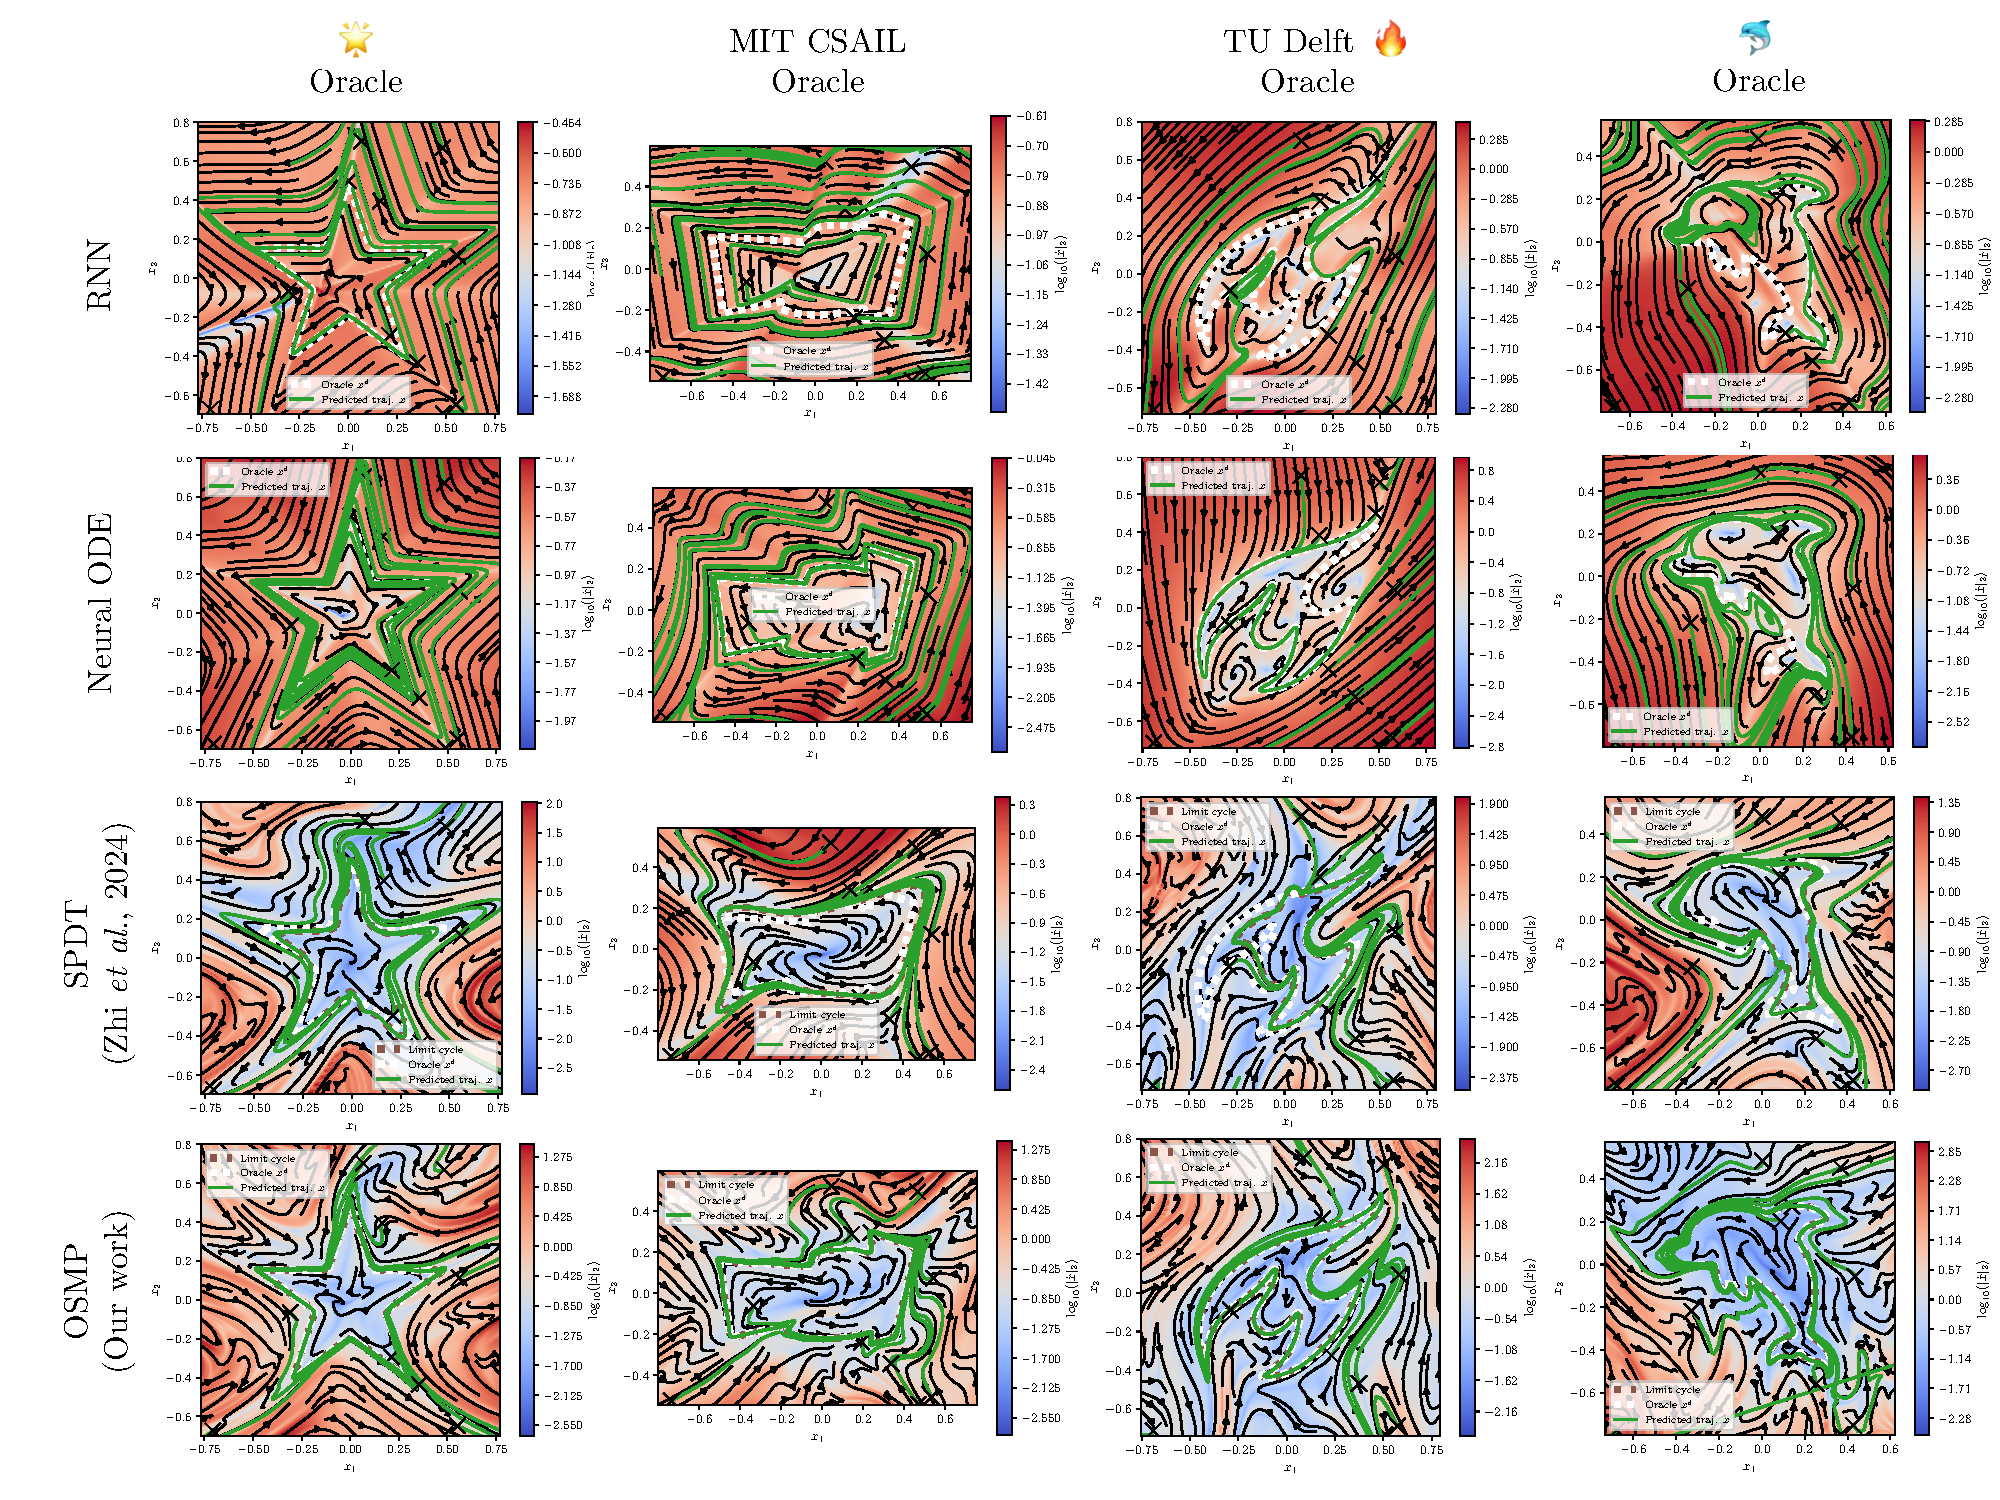
\includegraphics[width=1.0\linewidth]{osmp/figures/benchmarking_results/benchmarking_results_v1_cropped_compressed.pdf}
    \caption{\textbf{Benchmarking the oracle tracking performance and orbital stability of \glspl{OSMP}.}
    In this figure, we display the qualitative benchmarking results when comparing the proposed \gls{OSMP} against baseline methods, such as \glspl{RNN}, \glspl{NODE}~\citep{chen2018neural}, or \gls{SPDT}~\citep{zhi2024teaching}. The various columns represent different geometric shape-based oracles on which the motion policies were trained, shown as white dotted lines on the plots. The color map and the streamlines denote the velocity of the learned motion policy when evaluated on a grid. We initialize the trained motion policies at 10 different randomly sampled initial conditions and roll out their trajectory, visualized using solid green lines, for a duration of one period.
    }
    \label{fig:osmp:benchmarking_results}
\end{figure}

% The results presented in Fig.~\ref{fig:osmp:benchmarking_results} show that the proposed \gls{OSMP} exhibits superior convergence and stability characteristics compared to motion policies without physical structure, such as \glspl{RNN} or \glspl{NODE}. Specifically, for the relatively simple case of the star shape, most trajectories still converge to the periodic demonstration, but we notice some spurious attractors in the center of the star shape. For more complex oracles such as the TU Delft flame or the Dolphin oracle, the \gls{RNN} and the \gls{NODE} based motion policies are not able to track the demonstration in a stable fashion.
% While \gls{SPDT}~\citep{zhi2024teaching} exhibits the same stability and convergence guarantees as \gls{OSMP}, we notice a much-improved precision of \glspl{OSMP} at shaping the limit cycle such that it accurately matches the given periodic oracle. While this can already be noticed for the star oracle, this is particularly apparent for the TU Delft flame and Dolphin oracles.
The results in Fig.~\ref{fig:osmp:benchmarking_results} demonstrate that the proposed \gls{OSMP} offers superior convergence and stability compared to motion policies lacking physical structure, such as \glspl{RNN} or \glspl{NODE}. In the relatively simple case of the star shape, most trajectories converge to the periodic demonstration, although some spurious attractors appear inside the limit cycle. For more complex oracles, like the TU Delft flame or Dolphin shapes, the \gls{RNN}- and \gls{NODE}-based motion policies fail to track the demonstration in a stable fashion. While \gls{SPDT}~\citep{zhi2024teaching} provides similar stability and convergence guarantees to \gls{OSMP}, we observe that \gls{OSMP} achieves much higher precision in shaping the limit cycle to accurately match the given periodic oracle—a difference that is evident even in the star oracle and especially pronounced for the TU Delft flame and Dolphin oracles.

\subsection{Stable Tracking of Oracles Across Robot Embodiments}
% \begin{itemize}
%     \item Demonstrate how our proposed method is able to generate stable and accurate trajectories on a large variety of real-world robots.
%     \item Show experimental results for trajectory tracking on UR5 (robotic manipulator), KUKA (cobot), Helix (continuum soft robot), and joint-space and task-space turtle (rigid-soft underwater robot).
%     \item Possibly include comparisons with traditional trajectory tracking controllers to demonstrate that our learned motion primitive does not exhibit worse tracking accuracy.
% \end{itemize}

While the previous section focused on evaluating and benchmarking the learning of the \gls{OSMP}, we now aim to demonstrate that the proposed \gls{OSMP} can effectively control robot motion in real-world scenarios. To achieve this, we apply the method to a diverse range of robot embodiments, including robot manipulators (UR5), \glspl{Cobot} (KUKA), soft robots (Helix Robot)~\citep{guan2023trimmed}, and prototypes of hybrid soft-rigid underwater robots (Crush turtle robot).

\begin{figure}[h!]
    \centering
    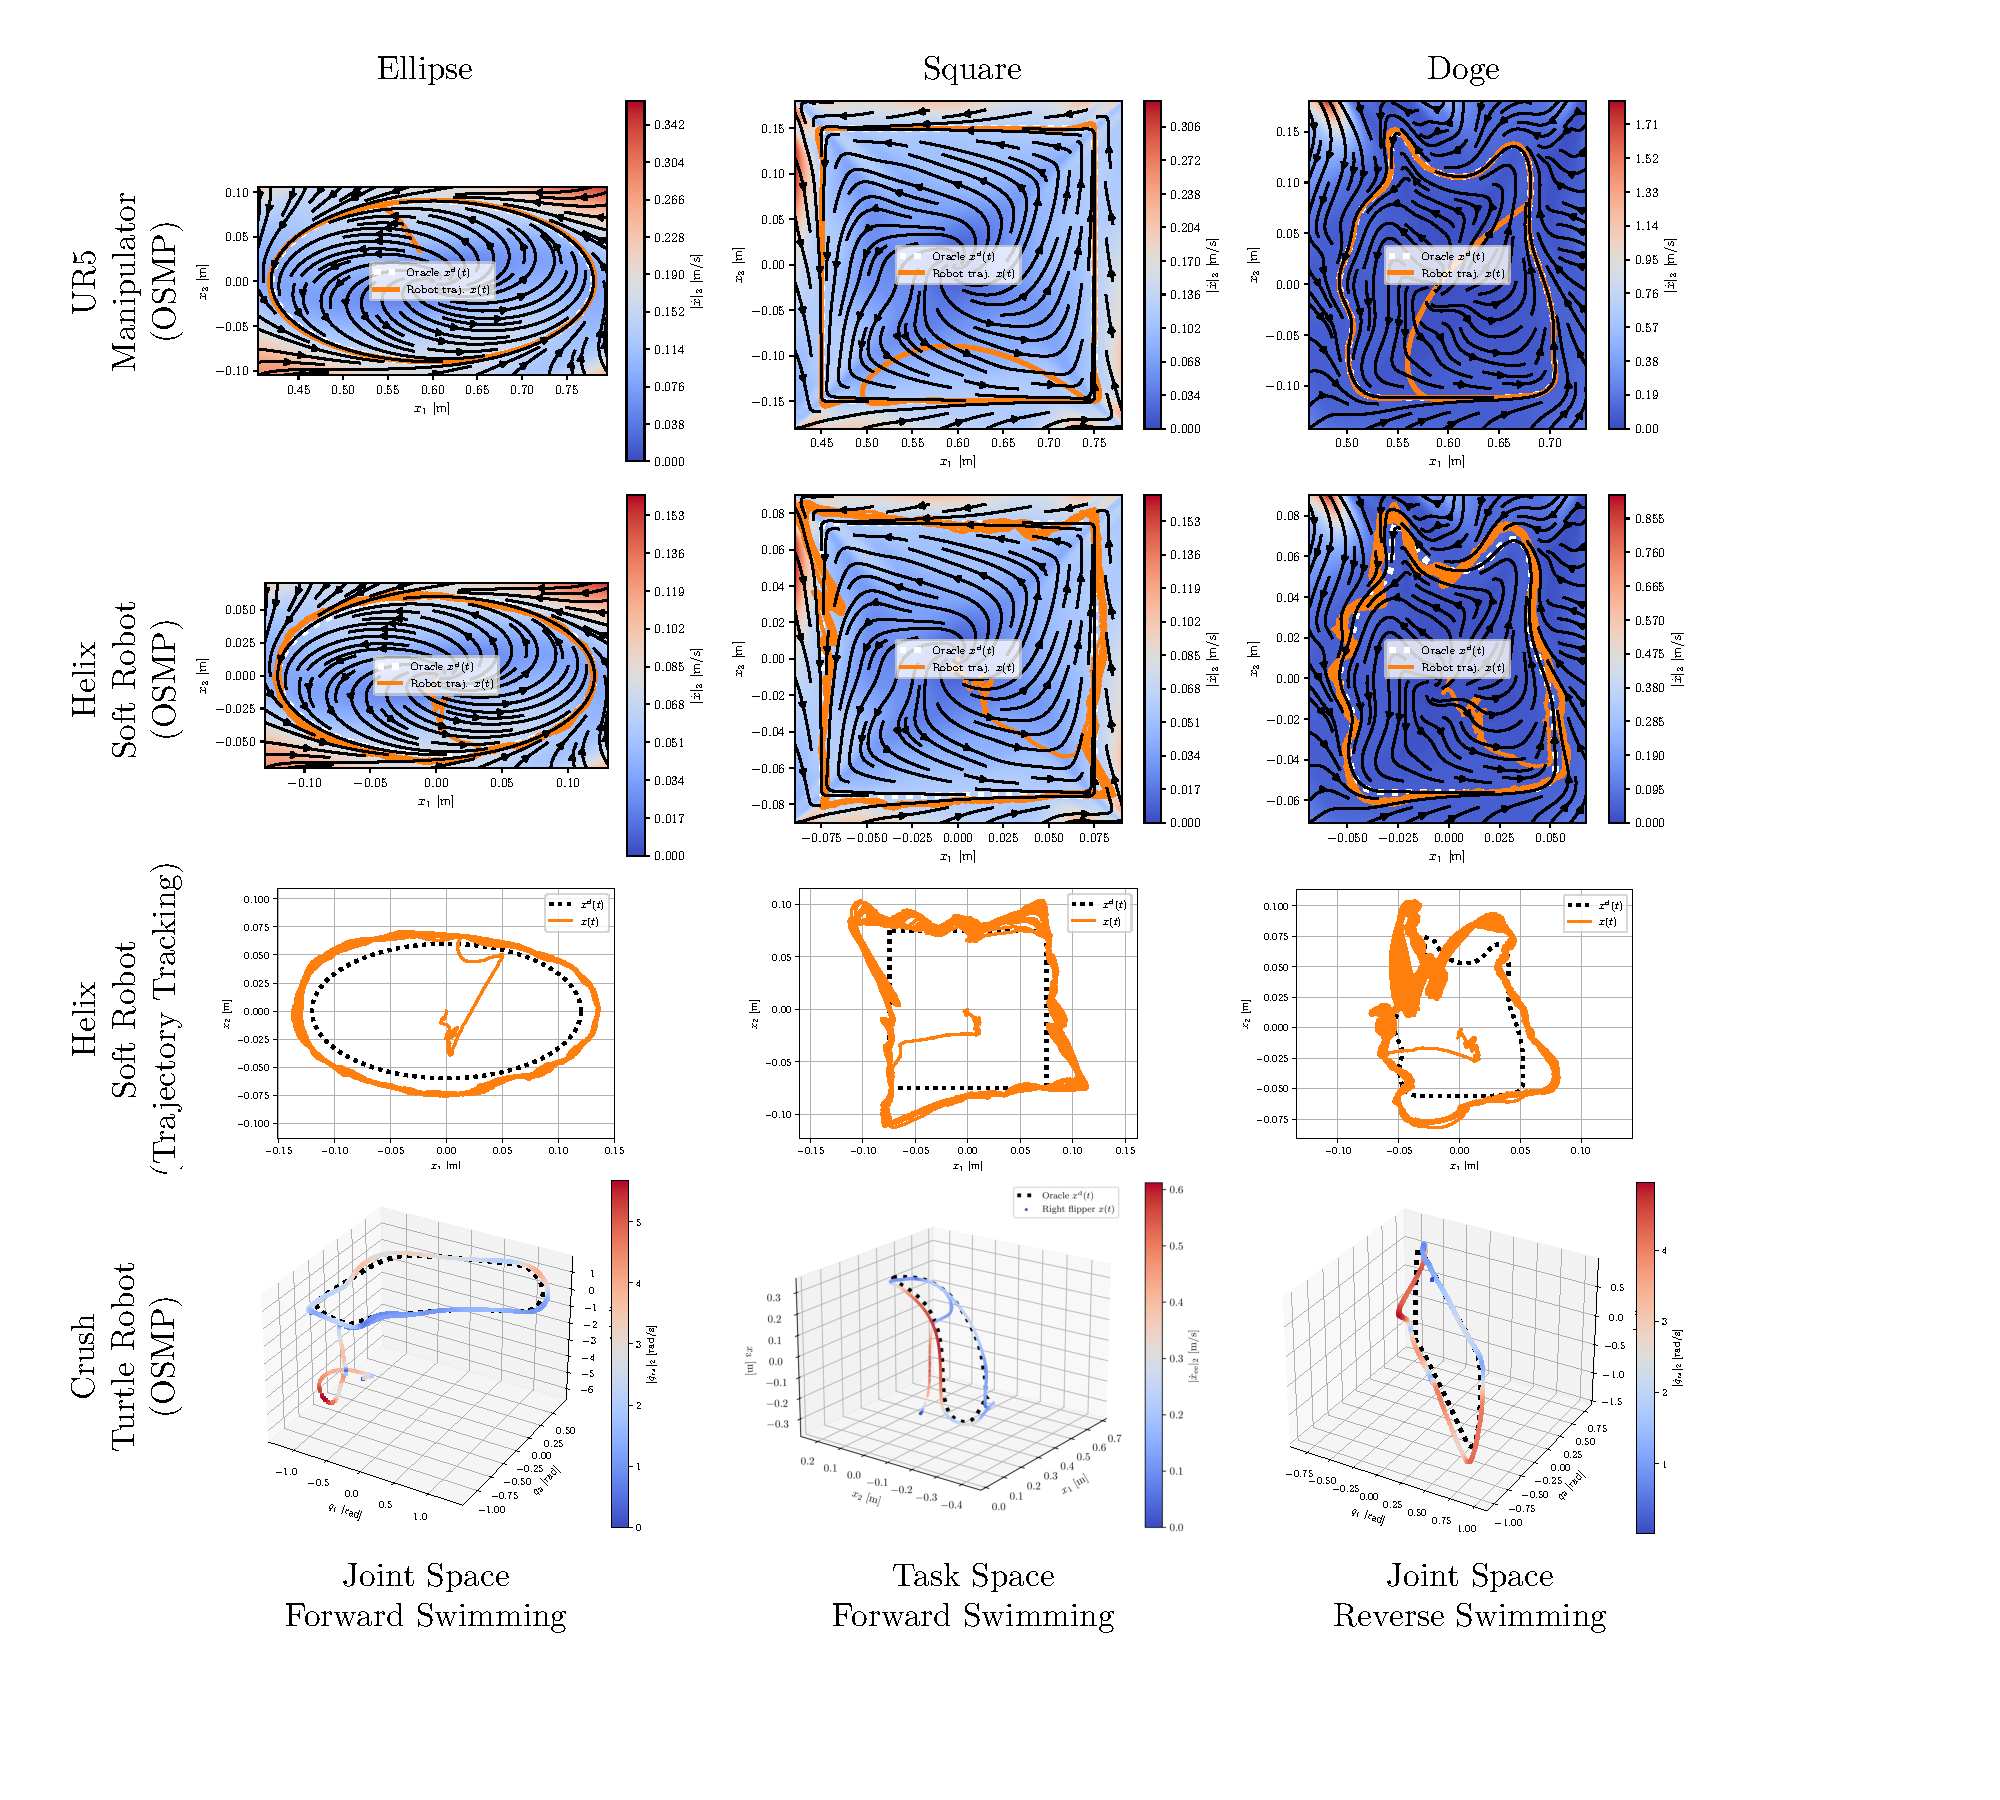
\includegraphics[width=1.0\linewidth]{osmp/figures/robot_embodiments_results/robot_embodiments_results_v1_cropped.pdf}
    \caption{\textbf{Stable tracking of oracles across robot embodiments in the real world.}
    This figure shows the trajectories of various robot embodiments controlled with \glspl{OSMP} based on data recorded during real-world experiments.
    The first row shows the behavior of a UR5 manipulator in task space where the \gls{OSMP} is trained on various geometric shape oracles, including an ellipse, a square, and a doge. The black dotted lines denote the oracle, the orange line is the actual trajectory of the UR5's end-effector, and the velocity field is based on the learned \gls{OSMP}.
    The second row considers the same trained \glspl{OSMP}, but this time evaluates their behavior on a Helix soft robot.
    The third row presents the behavior of traditional trajectory tracking controllers on the Helix soft robot for the same oracles.
    Finally, the fourth row contains measurements of the Crush turtle robot operated (in water) by \glspl{OSMP} trained on biological oracles, where the black dotted line denotes the oracle and the colored line the actual behavior of the right flipper arm. In the first and third, the forward swimming (biological)~\citep{van2022new} and reverse swimming oracles, respectively, are directly defined in joint space~\citep{van2023soft}. The second row shows a \gls{OSMP} applied to a biological forward swimming oracle defined in task space, which, in this case, corresponds to the tip position and twist angle (not visible here) of the right flipper arm.
    }
    \label{fig:osmp:robot_embodiments_results}
\end{figure}

Figure~\ref{fig:osmp:robot_embodiments_results} illustrates the effectiveness of OSMPs across all tested robot embodiments. 
% Here, the OSMP operates in task space and outputs desired task space velocities. Subsequently, we modify the robot's low-level controllers (task space) setpoint by incrementing the end effector position based on the desired velocity and the used time step.
Here, the OSMP operates in task space, outputting the desired task space velocities. Next, we update the robot’s low-level controller setpoint by incrementing the end effector’s position based on the desired velocity and the applied time step.
For the UR5 manipulator, we observe precise trajectory tracking. Although the Helix soft robot is also capable of tracking the trajectory, hysteresis effects and inaccuracies in its kinematic model—which lead to incorrect actuation inputs from the inverse kinematics—result in some oscillatory behavior and imprecision. It is important to note that this is not an inherent limitation of the \gls{OSMP} method but rather an issue that similarly affects traditional trajectory tracking methods, as it can be seen that the trajectory tracking controller, defined in \eqref{eq:osmp:trajectory_tracking_controller}, exhibits steady-state errors and in parts of the trajectory even instability.

In addition, we pursue learning swimming behavior for the Crush Turtle robot using biological oracles. Specifically, our objective is to have the \gls{OSMP} control the two front flipper arms—the primary tools for turtle swimming. We employ both a three-dimensional oracle defined in joint space~\citep{van2023soft} and a four-dimensional oracle defined in task space (comprising the flipper tip position and twist angle)~\citep{van2022new}, both derived from video recordings of green sea turtles (Chelonia mydas)~\citep{van2022new, van2023soft}. Subsequently, the commanded joint space velocities are tracked by the actuators.
These instances illustrate that \glspl{OSMP} can learn oracles with dimensions exceeding $n=2$. In real-world pool experiments, we observe that \glspl{OSMP} enable the Crush Turtle robot to accurately track the trajectory at moderate speeds. When the period of the periodic trajectory is shortened by increasing $\omega$, the motor’s acceleration and velocity constraints prevent perfect tracking, particularly during the faster segments of the oracle. Nonetheless, even if the motion diverges from the oracle, stability is maintained, and the system consistently returns to the oracle.

\begin{figure}
    \centering
    \includegraphics[width=1.0\linewidth]{osmp/figures/kinesthetic_teaching_results/kinesthetic_teaching_results_v1_cropped.pdf}
    \caption{\textbf{Real-world results for learning orbital motion primitives from kinesthetic oracles.}
    In the first column, we show the results for a whiteboard cleaning task executed with the UR5 manipulator, and in the second and third columns, we show the results for a booming task executed with the KUKA robot.
    In both cases, the demonstration was provided via kinesthetic teaching, and the \gls{OSMP} was trained on the resulting periodic oracle.
    For the UR5 manipulator, the \gls{OSMP} learns the motion of the end-effector position in three dimensions. For the KUKA manipulator, we learn both the motion of the end-effector position and orientation.
    The color signifies the time when executing the task using the trained \gls{OSMP}.
    }
    \label{fig:osmp:kinesthetic_teaching_results}
\end{figure}

\subsection{Learning Orbital Motion Primitives from Kinesthetic Oracles}
% \begin{itemize}
%     \item Demonstrate how our method is able to be applied to demonstrations that were created using kinesthetic teaching and that it is able to accomplish real-world tasks.
%     \item Show results for UR5 whiteboard cleaning and KUKA brooming tasks.
% \end{itemize}

In this section, we examine demonstrations captured through kinesthetic teaching, which tend to be more jerky and less smooth compared to the well-defined geometric oracles discussed earlier. Moreover, when demonstrating periodic motion, the oracle usually does not perfectly close, as a spatial offset remains between the starting and ending poses, which makes it more challenging to fit the limit cycle to the oracle accurately

In Fig.~\ref{fig:osmp:kinesthetic_teaching_results}, we present results for learning \glspl{OSMP} on cleaning tasks that were provided via kinesthetic teaching. Specifically, we consider a whiteboard erasure task on a UR5 manipulator and a brooming task on a KUKA cobot.
While in the case of the UR5, we only encode the spatial translation (i.e., positions) of the end-effector in the \gls{OSMP}, we also consider the motion of the end-effector orientation in the case of the KUKA task. 
In the case of the UR5 robot, we observe a fast convergence onto the limit cycle and, subsequently, good tracking of the oracle with only minor deviations at the point where we fused the start/end points of the periodic motions.
When deploying the \gls{OSMP} on the KUKA \gls{Cobot}, we notice a larger tracking error - likely due to the challenging oracle with $n=6$ \glspl{DOF} and the low feedback gains used in the low-level controller.


\begin{figure}[h]
    \centering
    \includegraphics[width=1.0\linewidth]{osmp/figures/compliance_results/compliance_results_v1_cropped.pdf}
    \caption{\textbf{Analyzing the compliance and motion behavior.}
    Simulations with time perturbations where we compare the behavior of traditional, time-parametrized trajectory tracking controllers against the \glspl{OSMP}. Here, the dashed black lines denote the oracles/demonstrations, the solid blue lines the behavior of a pure feedforward trajectory tracking controller $\dot{x}(t) = \dot{x}^\mathrm{d}(t)$ operating on a time-parametrized reference $\dot{x}^\mathrm{d}(t)$, the orange line the behavior of an error-based feedback trajectory tracking controller $\dot{x}(t) = \dot{x}^\mathrm{d}(t) + k_\mathrm{p} \, (x^\mathrm{d}(t) - x(t))$ with $k_\mathrm{p} = 1$, and the green line the behavior of the learned \gls{OSMP}. Compared to nominal scenarios, we perturb the time reference - i.e., the time reference exhibits a $\pi$ offset in phase with respect to the initial position.
    }
    \label{fig:osmp:compliance_results}
\end{figure}

\subsection{The Learned Policies Exhibit Compliant and Natural Motion Behavior}
% \begin{itemize}
%     \item The goal of this subsection is to show how a policy parametrized by a dynamic system is much more compliant and exhibits more natural and predictable motions than a traditional time-parametrized trajectory tracking controller.
%     \item Show a simulated 2D toy case where we perturb the time reference. Then, we compare the trajectories of a) a time-parametrized pure feedforward controller, b) a time-parametrized feedforward+feedback controller, and c) our orbital motion primitive. The feedforward controller would diverge upon time perturbation, the feedforward+feedback controller would be able to track the trajectory but exhibit unnatural motions, and the motion primitives are not affected by a perturbation in the time reference.
%     \item Show the results of the real-world experiments where the dynamical motion primitive exhibited a much more compliant behavior upon physical interaction of the robot than the time-parametrized trajectory tracking controller.
% \end{itemize}

We aim for robots in human-centric environments to demonstrate robust, compliant, and predictable behavior. Specifically, \emph{robustness} means that if a robot deviates from its intended path—perhaps due to a disturbance—it will always converge back to the desired motion. \emph{Compliance} indicates that robots should exert only minimal forces when coming into contact with humans, and \emph{predictability} ensures that their motions are sufficiently consistent for humans to anticipate their behavior and respond appropriately.

In this section, we compare the reaction upon disturbances and perturbations of \glspl{OSMP} against traditional trajectory tracking controllers that rely on a time-parametrized trajectory.
Such error-based feedback controllers are usually given in the form
\begin{equation}\label{eq:osmp:trajectory_tracking_controller}
    \dot{x}(t) = \dot{x}^\mathrm{d}(t) + K_\mathrm{p} \, (x^\mathrm{d}(t) - x(t)),
\end{equation}
where $K_\mathrm{p} \in \mathbb{R}^{n \times n}$ is a proportional feedback gain that operates on the error between the current position $x(t)$ and the desired position $x^\mathrm{d}(t)$. In practice, we choose a scalar $k_\mathrm{p} \in \mathbb{R}_+$ such that $K_\mathrm{p} = k_\mathrm{p} \, \mathbb{I}_{n}$. We stress here the reliance on a time-parametrized trajectory provided in the form $(x^\mathrm{d}(t),\dot{x}^\mathrm{d}(t)) \: \forall \: t \in [t_0, t_\mathrm{f}]$. 
We evaluate in simulation three motion controllers: a pure feedforward trajectory tracking controller, which we gather by setting $k_\mathrm{p} = 0$, and an error-based feedback controller with $k_\mathrm{p} > 0$, and the learned \gls{OSMP}.
In this setting, we are particularly interested in analyzing the behavior of the motion controllers upon encountering an external disturbance that perturbs the state of the system with respect to the time reference. For this, we shift the time reference when initializing the system by half a period (i.e., a phase shift of $\pi$~rad).

The results in Fig.~\ref{fig:osmp:compliance_results} show that the pure feedforward trajectory tracking controller entirely drifts off the desired trajectory. When adding an error-based feedback term, the traditional trajectory tracking controller is able to recover and rejoin the demonstrated trajectory after a bit. However, while doing so, the feedback term generates a very aggressive correction action, which could cause incompliant behavior and would not seem natural to humans. Instead, the \gls{OSMP}, which is solely conditioned on the system state and not time, is not affected by the perturbation of the time reference and perfectly tracks the demonstration while exhibiting compliant and natural behavior.


\subsection{Achieving Phase Synchronization Across Multiple Motion Primitives}
% \begin{itemize}
%     \item Motivate why phase synchronization is important and for which applications it can be useful.
%     \item Showcase a 2D toy example where we are synchronizing three or more learned motion primitives.
%     \item Show the real-world results from the turtle pool tests where i) the turtle doesn't swim when the flippers are not synchronized, ii) how we achieve the flipper synchronization and how that makes the turtle swim.
% \end{itemize}

In many practical applications, such as locomotion, synchronizing multiple motion policies is critical. In this section, we illustrate how our approach can synchronize multiple learned \glspl{OSMP} by evaluating the polar phase of each and then aligning them via an error-based feedback controller~\citep{dorfler2014synchronization}. Crucially, we only adjust the velocity magnitude without altering the system’s spatial motion, thereby preserving the imitation and convergence properties of each learned motion policy.

\begin{figure}[h]
    \centering
    \includegraphics[width=1.0\linewidth]{osmp/figures/phase_sync_results/phase_sync_results_v1_cropped.pdf}
    \caption{\textbf{Phase synchronization of \glspl{OSMP}.}
    Results for the phase synchronization of multiple \gls{OSMP} systems. The first row shows the Cartesian-space evolution of each \gls{OSMP}, where the color of the markers communicates the time information. The second row shows the position vs. time, and the last row shows the polar phase $\varphi$ of the systems over time. 
    The first three columns show simulation results for \glspl{OSMP} trained on ellipse and Dolphin demonstrations, respectively. In all rows, we synchronize the motion of two systems/\glspl{OSMP}, except for the third row, where we synchronize four systems.
    }
    \label{fig:osmp:phase_sync_results}
\end{figure}

In Fig.~\ref{fig:osmp:phase_sync_results}, we show simulation and experimental results for synchronizing two and four \glspl{OSMP}. The outcomes illustrate how the controller identifies the most efficient strategy to align the \glspl{OSMP}, achieving rapid polar phase synchronization. A proportional gain determines the aggressiveness of the synchronization process. The simulation results confirm that the phase synchronization approach is effective not only for two systems but also for four or more.

Regarding experimental findings, we examined the swimming performance of the Crush turtle robot. Tests in a swimming pool revealed that the robot can swim effectively only when both front flippers—the primary means of locomotion in water~\citep{van2022new, van2023soft}—are fully synchronized. In practice, even aside from external disturbances and inherent differences between the flippers, desynchronization occurs already during initialization when the flipper arms start in slightly different configurations with varying polar phases. Our results show that using our method, the two flipper arms synchronize in less than a quarter of a period, thereby enabling the turtle robot to swim effectively.

\subsection{Smooth Interpolation Between Oracles via Encoder Conditioning}
% \begin{itemize}
%     \item Motivate how encoder conditioning enables the incorporation of multiple oracles in the same motion primitive.
%     \item Motivate why we would (ideally) want to achieve smooth interpolation between oracles.
%     \item Showcase 2D toy examples for the interpolation between two or more oracles. We also show that this works in the real world on the UR5 robot.
%     \item Demonstrate how we can learn both forward and reverse turtle swimming with the same motion primitive using encoder conditioning and how we can smoothly interpolate between the two motions.
% \end{itemize}

As we move toward generalist motion policies~\citep{o2024open, black2024pi0, gemini2025robotics}, the motion policy must integrate not just a single behavior but a range of diverse behaviors conditioned on the task, the robot’s state, and its perception of the environment. In particular, we aim to leverage in the future semantic encodings from sources like \glspl{VLM} as motion conditioning. However, this aspect has not been sufficiently explored within the realm of dynamic motion primitives. Moreover, there may be many scenarios where interpolating between two or more motion behaviors from the training set is beneficial, which is not supported by the current methods~\citep{rana2020euclideanizing, perez2023stable, perez2024puma, sochopoulos2024learning, zhi2024teaching}.
%
One example involves different surface cleaning motions, where the specific cleaning action is selected based on the surface material. In this case, the robot should be able to transition smoothly between cleaning motions when moving from one surface to another. Another example is locomotion: if oracles are available for walking on flat terrain and for stepping over steep stairs, then for obstacles or moderately steep, stair-like terrain, it may be beneficial to interpolate between these two oracles, while we would want to preserve the naturalness of the motion.

\begin{figure}[h]
    \centering
    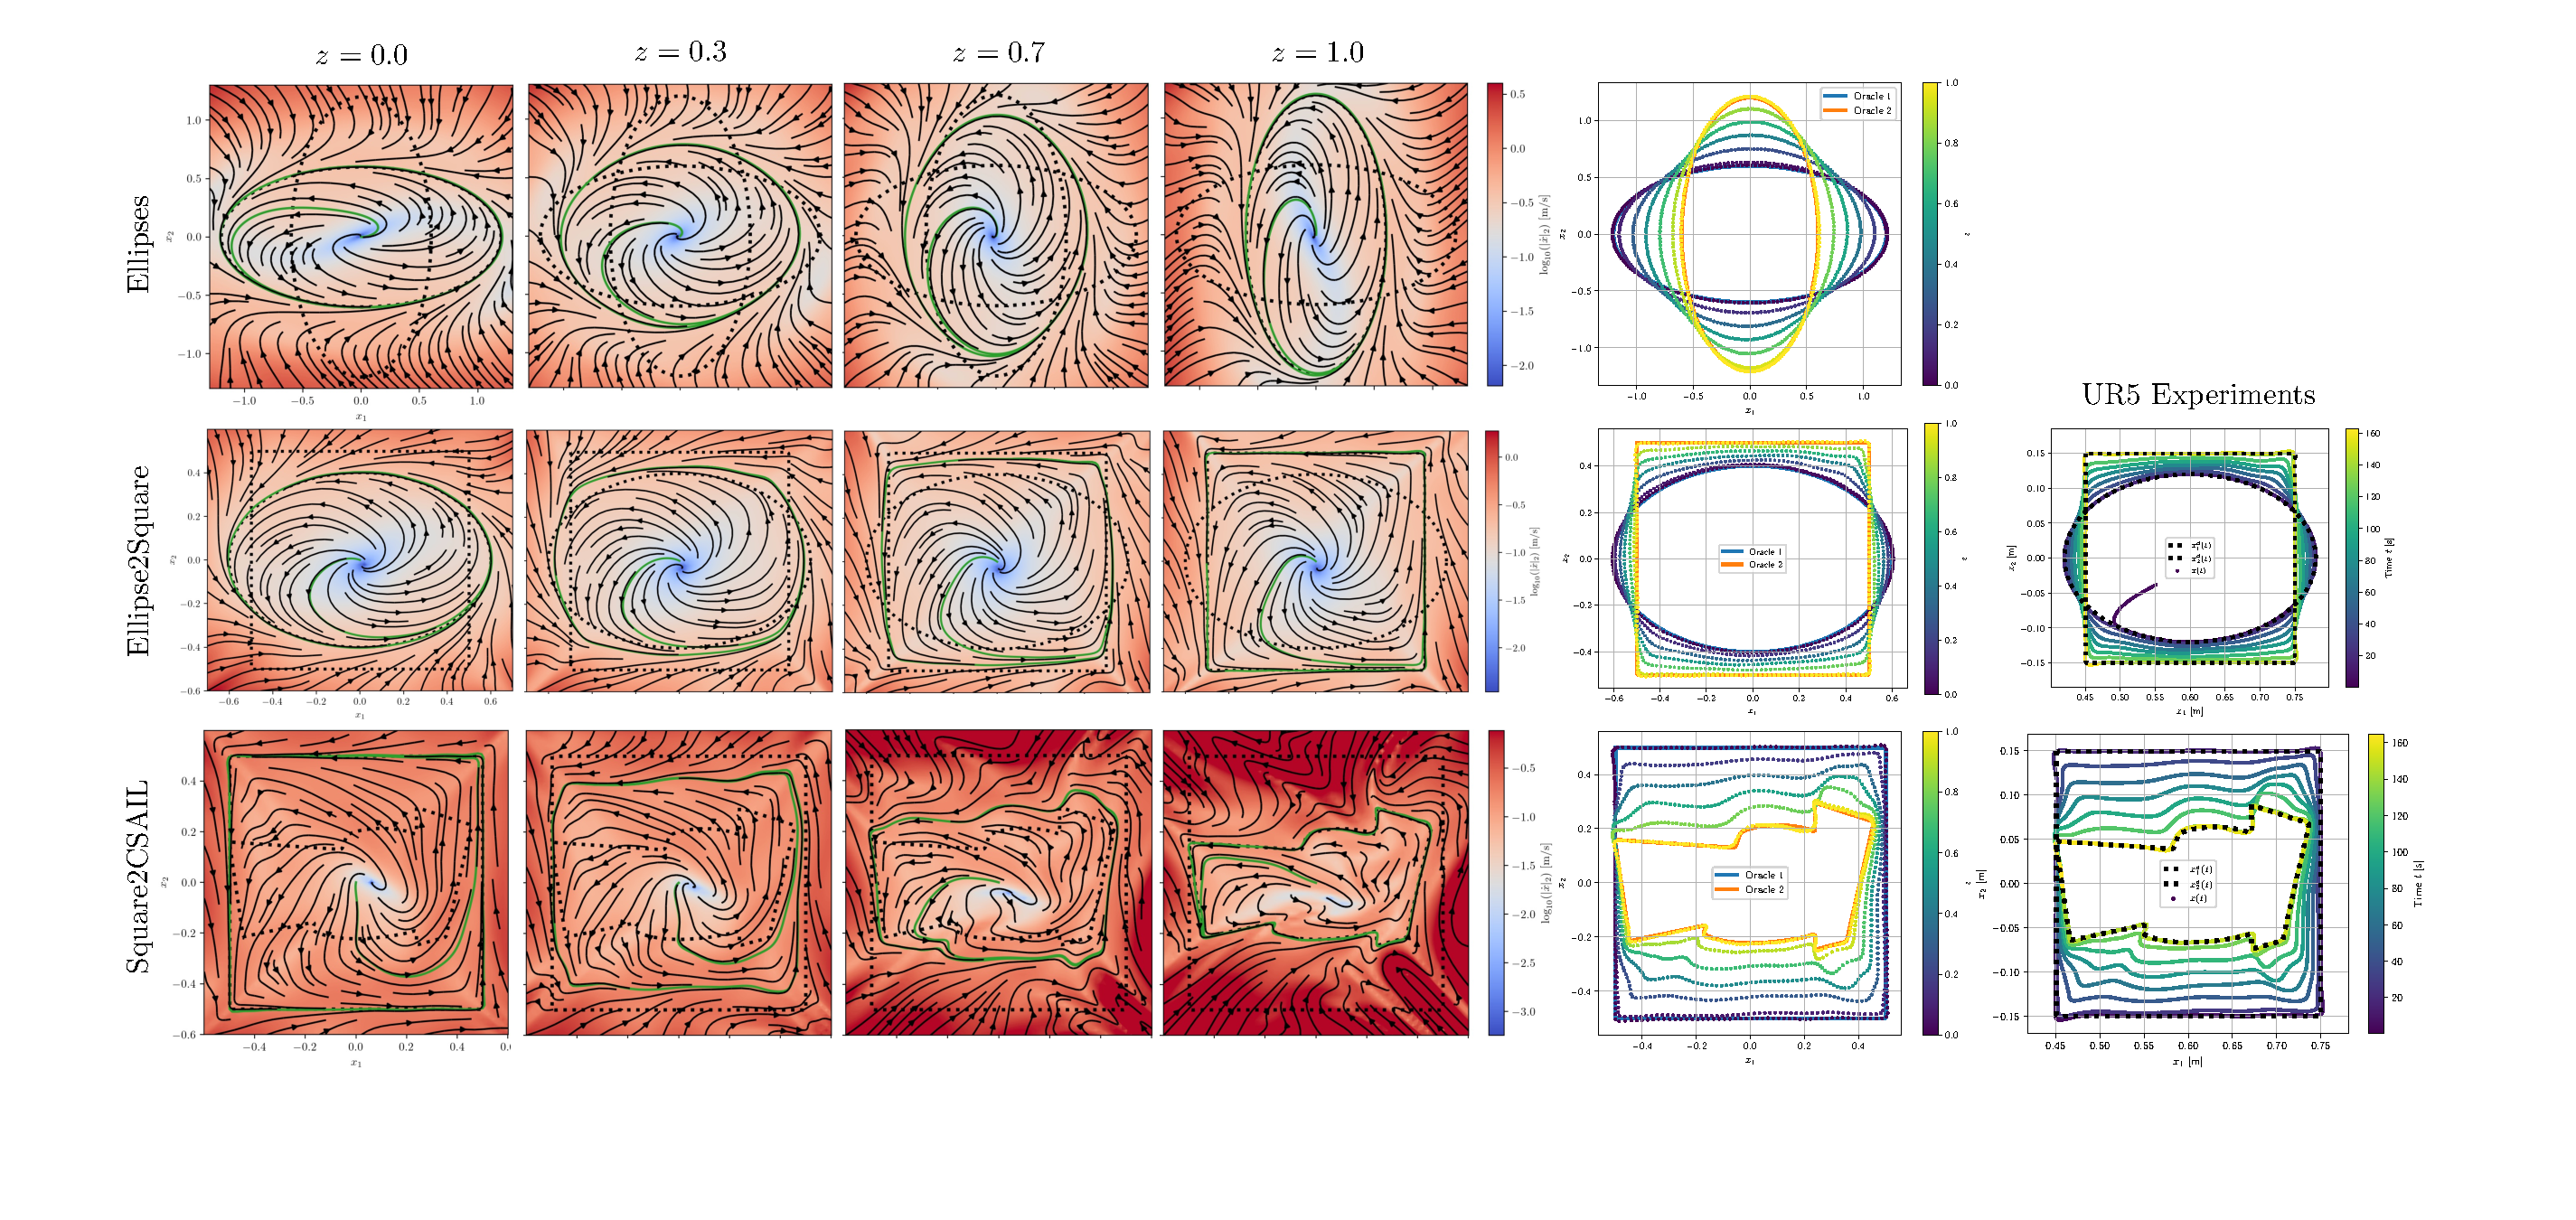
\includegraphics[width=1.0\linewidth]{osmp/figures/conditioning_results/conditioning_results_v1_cropped.pdf}
    \caption{
    \textbf{Smooth interpolation between distinct motion behaviors via encoder conditioning.}
    Results demonstrating the conditioning of the encoder on multiple learned motion behaviors, including smooth interpolation between behaviors.
    The first row shows the behavior of an OSMP that was trained jointly on a horizontal ellipse ($z=0$) and a vertical ellipse ($z=1$).
    The second row shows the behavior of an OSMP that was trained jointly on a horizontal ellipse ($z=0$) and a square ($z=1$).
    The third row shows the behavior of an OSMP that was trained jointly on a square ($z=0$) and the MIT CSAIL logo ($z=1$).
    The first four columns present the simulated behavior for a constant conditioning $z$ between $z=0$ and $z=1$, where the black dashed line denotes the two oracles used for training and the green line the simulated trajectory that is a function of the velocity field for the given conditioning $z$.
    The fifth column contains a simulation where the conditioning is slowly increased, where the color indicates the conditioning $z$.
    Similarly, the sixth column includes real-world results obtained with a UR5 manipulator where the conditioning is slowly increased from $z=0$ at $t=0$ to $z=1$ at $t=140$~s. Here, the color indicates the time.
    }
    \label{fig:osmp:conditioning_results}
\end{figure}

In this work, we introduce task conditioning for the bijective encoder using a conditioning variable $z \in \mathbb{R}$. This variable enables us to select the desired motion behavior online by providing the appropriate $z$ value. Moreover, we train the \gls{OSMP} so that the learned motion policy smoothly interpolates between two or more motion behavior conditionings (e.g., $z=0$ and $z=1$). As shown in Fig.~\ref{fig:osmp:conditioning_results}, our simulations and real-world experiments with a UR5 manipulator demonstrate that (a) the same \gls{OSMP} can accurately learn multiple motion behaviors and (b) smooth interpolation between these behaviors is achievable by adjusting the conditioning. Importantly, switching between motion behaviors does not require an elaborate sequence; once a new $z$ is set, the \gls{OSMP}’s convergence guarantees ensure that the system quickly adapts to the new behavior.
\section{Conclusion}
% In this chapter, we presented an approach for learning periodic/cyclical motion from demonstration using \glspl{OSMP}, where the motion policy is, analog to \glspl{DMP}~\cite{ijspeert2002learning, ijspeert2013dynamical}, parametrized by a dynamical system.
% Specifically, we combined the strengths of \gls{ML} approaches, such as expressiveness and the lack of requirements for heuristics, with nonlinear system theory to guarantee that the periodic is tracked via a limit cycle behavior that exhibits orbital stability.
% We achieve this by combining a learned bijective encoder based on Euclideanizing flows~\citep{dinh2016density, rana2020euclideanizing} that establishes a diffeomorphism between the oracle and the latent space and inspectable and fixed dynamics in latent space given by supercritical Hopf birfurcation~~\cite{strogatz2018nonlinear}.
% Compared to existing work~\cite{zhi2024teaching}, we significantly improve the accuracy of the matching between periodic demonstration and the generated limit cycle.
% Additionally, we benchmark the \glspl{OSMP} against standard \gls{ML} methods which reveals that they guarnatee convergence while standard \gls{ML} methods such as \glspl{MLP} or \glspl{RNN} often exhibit spurious attractors.
% Also, we extensively validate the proposed method in the real-world on various robot embodiments, including robotic manipulators and \glspl{Cobot}, soft robots, and bioinspired hybrid soft-rigid underwater robots.
In this chapter, we introduced an approach for learning periodic/cyclical motions from demonstrations using \glspl{OSMP}, where—similar to \glspl{DMP}~\citep{ijspeert2002learning, ijspeert2013dynamical}—the motion policy is parametrized by a dynamical system. We combined the advantages of \gls{ML} methods, such as their high expressiveness, with nonlinear system theory to ensure that the periodic motion is tracked via a limit cycle that exhibits \glsxtrfull{OS}. This is achieved by integrating a learned bijective encoder based on Euclideanizing flows~\citep{dinh2016density, rana2020euclideanizing}, which establishes a diffeomorphism between the oracle and latent space, with fixed, inspectable dynamics in latent space provided by a supercritical Hopf bifurcation~\citep{strogatz2018nonlinear}. Compared to previous work~\citep{zhi2024teaching}, our approach significantly improves the accuracy of matching the periodic demonstration to the generated limit cycle. Furthermore, benchmarking against standard \gls{ML} techniques shows that \glspl{OSMP} guarantee convergence, whereas traditional methods such as \glspl{RNN} and \glspl{NODE}~\citep{zhi2024teaching} often exhibit spurious attractors. We also validate our method extensively in real-world settings across various robotic platforms, including robotic manipulators and \glspl{Cobot}, soft robots, and bioinspired hybrid soft-rigid underwater robots.

% Moreover, we devise several techniques that increase the capability of dynamic motion primitives, including online reshaping of the velocity field that adjust the convergence characteristics as needed without requiring retraining, the synchronization of multiple \glspl{OSMP} in their phase by leveraging a error-based feedback term, and the capability to learn several distinct motion behaviors with the same motion policy by conditioning the encoder on the task/motion behavior. After adding a loss term, we are even able to smoothly interpolate between two motion behaviors. 
Moreover, we developed several techniques to enhance the capabilities of dynamic motion primitives. These include online reshaping of the velocity field to adjust convergence characteristics without retraining, synchronizing multiple \glspl{OSMP} in phase via an error-based feedback term, and enabling the same motion policy to learn multiple distinct behaviors by conditioning the encoder on the task. With the addition of a tailored loss term, we can even achieve smooth interpolation between two motion behaviors.

% For future work, it would be interesting to allow the same motion primitive to exhibit multiple classes of attractors~\citep{strogatz2018nonlinear}, including \gls{GAS} (for point-to-point motions), \gls{MS} (for multiple goals with equal value), and \gls{OS} (for periodic motions).
% A first step would be to build on top of the formulation employed in this paper, as the supercritical Hopf bifurcation can capture both exhibit a single, isolated equilibrium and limit cycle behavior if we were to add an additional parameter that would allow us to control that~\citep{strogatz2018nonlinear}.
% Furthermore, it seems timely and obvious, to condition the encoder on the outputs/embeddings of modern \glspl{VLM}~\citep{o2024open, touvron2023llama, grattafiori2024llama}, which would allow to significantly increase the generalization, reasoning, and planning capabilities of the motion policies while preserving the insight, robustness, compliance, and convergence guarantees that \glspl{DMP} exhibit.
For future work, it would be intriguing to enable a single motion primitive to exhibit multiple classes of attractors~\citep{strogatz2018nonlinear}, such as \gls{GAS} for point-to-point motions, \gls{MS} for multiple equally valued goals, and \gls{OS} for periodic motions. An initial step could build on the formulation presented here, as the supercritical Hopf bifurcation can capture both a single isolated equilibrium and limit cycle behavior if an additional \emph{attractor type} parameter is introduced. Furthermore, it appears timely to condition the encoder on the outputs or embeddings of modern \glspl{VLM}~\citep{o2024open, touvron2023llama, grattafiori2024llama}, which would significantly enhance the generalization, reasoning, and planning capabilities of the motion policies while preserving the insight, robustness, compliance, and convergence guarantees inherent to \glspl{DMP}.
